% Options for packages loaded elsewhere
\PassOptionsToPackage{unicode}{hyperref}
\PassOptionsToPackage{hyphens}{url}
\PassOptionsToPackage{dvipsnames,svgnames,x11names}{xcolor}
%
\documentclass[
  12pt,
]{article}
\usepackage{amsmath,amssymb}
\usepackage{setspace}
\usepackage{iftex}
\ifPDFTeX
  \usepackage[T1]{fontenc}
  \usepackage[utf8]{inputenc}
  \usepackage{textcomp} % provide euro and other symbols
\else % if luatex or xetex
  \usepackage{unicode-math} % this also loads fontspec
  \defaultfontfeatures{Scale=MatchLowercase}
  \defaultfontfeatures[\rmfamily]{Ligatures=TeX,Scale=1}
\fi
\usepackage{lmodern}
\ifPDFTeX\else
  % xetex/luatex font selection
    \setmainfont[]{Helvetica}
\fi
% Use upquote if available, for straight quotes in verbatim environments
\IfFileExists{upquote.sty}{\usepackage{upquote}}{}
\IfFileExists{microtype.sty}{% use microtype if available
  \usepackage[]{microtype}
  \UseMicrotypeSet[protrusion]{basicmath} % disable protrusion for tt fonts
}{}
\makeatletter
\@ifundefined{KOMAClassName}{% if non-KOMA class
  \IfFileExists{parskip.sty}{%
    \usepackage{parskip}
  }{% else
    \setlength{\parindent}{0pt}
    \setlength{\parskip}{6pt plus 2pt minus 1pt}}
}{% if KOMA class
  \KOMAoptions{parskip=half}}
\makeatother
\usepackage{xcolor}
\usepackage[margin=2cm]{geometry}
\usepackage{longtable,booktabs,array}
\usepackage{calc} % for calculating minipage widths
% Correct order of tables after \paragraph or \subparagraph
\usepackage{etoolbox}
\makeatletter
\patchcmd\longtable{\par}{\if@noskipsec\mbox{}\fi\par}{}{}
\makeatother
% Allow footnotes in longtable head/foot
\IfFileExists{footnotehyper.sty}{\usepackage{footnotehyper}}{\usepackage{footnote}}
\makesavenoteenv{longtable}
\usepackage{graphicx}
\makeatletter
\newsavebox\pandoc@box
\newcommand*\pandocbounded[1]{% scales image to fit in text height/width
  \sbox\pandoc@box{#1}%
  \Gscale@div\@tempa{\textheight}{\dimexpr\ht\pandoc@box+\dp\pandoc@box\relax}%
  \Gscale@div\@tempb{\linewidth}{\wd\pandoc@box}%
  \ifdim\@tempb\p@<\@tempa\p@\let\@tempa\@tempb\fi% select the smaller of both
  \ifdim\@tempa\p@<\p@\scalebox{\@tempa}{\usebox\pandoc@box}%
  \else\usebox{\pandoc@box}%
  \fi%
}
% Set default figure placement to htbp
\def\fps@figure{htbp}
\makeatother
\setlength{\emergencystretch}{3em} % prevent overfull lines
\providecommand{\tightlist}{%
  \setlength{\itemsep}{0pt}\setlength{\parskip}{0pt}}
\setcounter{secnumdepth}{5}
% definitions for citeproc citations
\NewDocumentCommand\citeproctext{}{}
\NewDocumentCommand\citeproc{mm}{%
  \begingroup\def\citeproctext{#2}\cite{#1}\endgroup}
\makeatletter
 % allow citations to break across lines
 \let\@cite@ofmt\@firstofone
 % avoid brackets around text for \cite:
 \def\@biblabel#1{}
 \def\@cite#1#2{{#1\if@tempswa , #2\fi}}
\makeatother
\newlength{\cslhangindent}
\setlength{\cslhangindent}{1.5em}
\newlength{\csllabelwidth}
\setlength{\csllabelwidth}{3em}
\newenvironment{CSLReferences}[2] % #1 hanging-indent, #2 entry-spacing
 {\begin{list}{}{%
  \setlength{\itemindent}{0pt}
  \setlength{\leftmargin}{0pt}
  \setlength{\parsep}{0pt}
  % turn on hanging indent if param 1 is 1
  \ifodd #1
   \setlength{\leftmargin}{\cslhangindent}
   \setlength{\itemindent}{-1\cslhangindent}
  \fi
  % set entry spacing
  \setlength{\itemsep}{#2\baselineskip}}}
 {\end{list}}
\usepackage{calc}
\newcommand{\CSLBlock}[1]{\hfill\break\parbox[t]{\linewidth}{\strut\ignorespaces#1\strut}}
\newcommand{\CSLLeftMargin}[1]{\parbox[t]{\csllabelwidth}{\strut#1\strut}}
\newcommand{\CSLRightInline}[1]{\parbox[t]{\linewidth - \csllabelwidth}{\strut#1\strut}}
\newcommand{\CSLIndent}[1]{\hspace{\cslhangindent}#1}
\usepackage[utf8]{inputenc}

% Break sections into new page
\usepackage{titlesec}
\newcommand{\sectionbreak}{\clearpage}
\usepackage{soul} % \hl{} = highlights

% Table caption 
\usepackage{caption} 
\captionsetup[table]{skip=8pt}

% Table packages
\usepackage{longtable}
\usepackage{array}
\usepackage{multirow}
\usepackage{wrapfig}
\usepackage{float}
\usepackage{colortbl}
\usepackage{pdflscape}
\usepackage{tabu}
\usepackage{threeparttable}
\usepackage{threeparttablex}
\usepackage[normalem]{ulem}
\usepackage{makecell}
\usepackage{xcolor}

% Move all figures at the end
\usepackage[nolists, nomarkers]{endfloat}
\DeclareDelayedFloatFlavour*{longtable}{table}

%\graphicspath{}

\usepackage{booktabs}
\usepackage{longtable}
\usepackage{array}
\usepackage{multirow}
\usepackage{wrapfig}
\usepackage{float}
\usepackage{colortbl}
\usepackage{pdflscape}
\usepackage{tabu}
\usepackage{threeparttable}
\usepackage{threeparttablex}
\usepackage[normalem]{ulem}
\usepackage{makecell}
\usepackage{xcolor}
\usepackage{bookmark}
\IfFileExists{xurl.sty}{\usepackage{xurl}}{} % add URL line breaks if available
\urlstyle{same}
\hypersetup{
  pdftitle={AI Chatbots in K-12 Education: An Experimental Study of Socratic vs.~Non-Socratic Approaches and the Role of Step-by-Step Reasoning},
  pdfauthor={Andrea Blasco1,; Vicky Charisi1,2,},
  colorlinks=true,
  linkcolor={Maroon},
  filecolor={Maroon},
  citecolor={Blue},
  urlcolor={Blue},
  pdfcreator={LaTeX via pandoc}}

\title{AI Chatbots in K-12 Education: An Experimental Study of Socratic vs.~Non-Socratic Approaches and the Role of Step-by-Step Reasoning}
\author{Andrea Blasco\textsuperscript{1,*} \and Vicky Charisi\textsuperscript{1,2,*}}
\date{This version: June 03, 2025}

\begin{document}
\maketitle

\setstretch{1.5}
\textsuperscript{1} European Commission, Joint Research Centre, Brussels, Belgium\\
\textsuperscript{2} Harvard University, Berkman Klein Center, Cambridge, MA, USA

\textsuperscript{*} Correspondence: \href{mailto:andrea.blasco@ec.europa.eu}{Andrea Blasco \textless{}\href{mailto:andrea.blasco@ec.europa.eu}{\nolinkurl{andrea.blasco@ec.europa.eu}}\textgreater{}}, \href{mailto:vcharisi@law.harvard.edu}{Vicky Charisi \textless{}\href{mailto:vcharisi@law.harvard.edu}{\nolinkurl{vcharisi@law.harvard.edu}}\textgreater{}}

\section*{Highlights}\label{highlights}
\addcontentsline{toc}{section}{Highlights}

\begin{itemize}
\item
  An experiment was conducted where K-12 students (N=122) used AI chatbots to solve school-related problems.
\item
  Two interventions were tested: (1) comparing AI-generated step-by-step explanations to predictions alone, and (2) contrasting AI chatbot support inspired by the Socratic method (guided questioning) versus non-Socratic (direct answers) support.
\end{itemize}

\begin{itemize}
\item
  Participants performed better under step-by-step explanations. They also engaged more frequently with the Socratic AI, though this approach did not result in improved performance and retain of knowledge compared to the non-Socratic AI.
\item
  While students found interactions with the AI useful, they perceived the Socratic AI as less helpful than non-Socratic overall.
\item
  The findings highlight challenges in designing AI tutors that effectively foster critical thinking while maintaining student satisfaction, raising concerns about their adoption in educational settings.
\end{itemize}

\section*{Abstract}\label{abstract}
\addcontentsline{toc}{section}{Abstract}

How does integrating large language models (LLMs) into classroom activities influence students' learning? To investigate this question, we conducted a randomized experiment with students aged 14-16 (N=122), testing two interventions: (i) comparing AI-generated solutions with step-by-step explanations versus solutions alone and (ii) Socratic AI chatbots promoting critical thinking through incremental guidance versus non-Socratic AI offering direct solutions. Students completed school-related tasks under these conditions. We collected students' performance and interaction logs data, as well as their attitudes through self-reported surveys. Results indicated that AI-generated explanations significantly improved students' performance over solutions alone, highlighting the benefits of step-by-step guidance. The Socratic AI approach fostered significantly greater engagement and interaction. However, it did not achieve significant improvements in learning, and a higher fraction of students perceived it as less helpful. Furthermore, despite overall positive perceptions of AI assistance, students exhibited limited retention, failing to apply learned concepts to new situations without the aid of AI. These findings underscore both the potential and limitations of LLM-based chatbots in K-12 education, especially in balancing the development of critical thinking with user satisfaction.

\textbf{Keywords}: artificial intelligence; large language models; learning; education policy; experiment; k-12

\section{Introduction}\label{introduction}

Integrating artificial intelligence (AI) into educational settings has been debated for over three decades (\citeproc{ref-roll2016evolution}{Roll and Wylie 2016}). Recent advances in generative AI and large language model (LLM) chatbots have opened even more possibilities for improvements in educational practices (\citeproc{ref-yan2024promises}{Yan, Greiff, et al. 2024}; \citeproc{ref-kasneci2023chatgpt}{Kasneci et al. 2023}; \citeproc{ref-tlili2023if}{Tlili et al. 2023}; \citeproc{ref-debets2025chatbots}{Debets et al. 2025}). Although LLMs mimic human intelligence, their applications extend beyond imitation and include a range of academic tasks: facilitating problem-solving (\citeproc{ref-urban2024chatgpt}{Urban et al. 2024}), providing personalised assistance (\citeproc{ref-darvishi2024impact}{Darvishi et al. 2024}), language learning (\citeproc{ref-derakhshan2024chatgpt}{Derakhshan and Ghiasvand 2024}; \citeproc{ref-song2023enhancing}{Song and Song 2023}), and evaluating students' work (\citeproc{ref-henkel2024can}{Henkel et al. 2024}). However, the impact of these applications on students' learning remains controversial, with proponents highlighting potential benefits and critics cautioning about risks and drawbacks (\citeproc{ref-farrokhnia2024swot}{Farrokhnia et al. 2024}; \citeproc{ref-weidinger2022taxonomy}{Weidinger et al. 2022}; \citeproc{ref-walczak2023challenges}{Walczak and Cellary 2023}).

A key advancement over previous AI systems is that LLMs can provide step-by-step reasoning to answer students' queries (\citeproc{ref-wei2022chain}{Wei et al. 2022}) and that by adding ``Let's think step by step'\,`, LLMs can improve their performance significantly (\citeproc{ref-kojima2022large}{Kojima et al. 2022}). Although evidence suggests that such explanations can foster children's learning and contribute to the development of their scientific reasoning (\citeproc{ref-dejong1986explanation}{DeJong and Mooney 1986}; \citeproc{ref-legare2014contributions}{Legare 2014}; \citeproc{ref-danovitch2021mind}{Danovitch et al. 2021}), there is limited empirical research examining how such AI-generated explanations impact students' learning processes. Most prior studies have not isolated the specific role of detailed AI-generated reasoning in enhancing problem-solving skills. To fill this gap, we conducted a randomised experiment with k-12 students (n = 122) who were engaged in a simple estimation task -- guessing the value of coins in a jar. Half of the participants received only an AI-generated prediction, while the other half were additionally provided with AI-generated explanations detailing how to derive such estimation. This setup enabled to address our first research question (RQ):

\textbf{RQ1: Do AI-generated explanations enhance students' problem-solving performance in school tasks, specifically in terms of estimation accuracy?}

The distinction between AI-generated \emph{explanations} and \emph{solutions} further allows us to evaluate whether providing explanations influences students' trust and judgment of AI-generated content. Indeed, LLMs can generate inaccurate solutions and flawed reasoning (\citeproc{ref-saxton2019analysing}{Saxton et al. 2019}; \citeproc{ref-kalyan2021how}{Kalyan et al. 2021}; \citeproc{ref-hendrycks2021measuring}{Hendrycks et al. 2021}). However, there is evidence that providing explanations increases users' trust and acceptance of AI systems, especially when the reasoning behind the output is clear (\citeproc{ref-rai2020explainable}{Rai 2020}; \citeproc{ref-ferrario2022explainability}{Ferrario and Loi 2022}). In an educational setting, this may affect learning outcomes in a complex manner. Students may interpret well-written explanations as evidence that an answer is correct, even when it is not. Conversely, they may notice minor errors or inconsistencies in an explanation that reduce their trust, even if the overall solution is accurate. This situation motivates our second research question:

\textbf{RQ2: How do AI-generated explanations influence students' perceived credibility of AI-generated solutions?}

Another critical technical progress of contemporary LLMs over previous AI systems is their ability to follow specific instructions when engaged in conversations. Building on this capability, another goal of this study is to examine the impact of two fundamental modes of interaction on students' learning outcomes: one that fosters critical thinking through incremental guidance (``Socratic AI'') and another that offers immediate solutions (``non-Socratic AI'').

Although classical pedagogical methods, such as the Socratic Method, have long been valued for promoting critical thinking and a deeper understanding (\citeproc{ref-lam2011socratic}{Lam 2011}; \citeproc{ref-dalim2022promoting}{Dalim, Ishak, and Hamzah 2022}; \citeproc{ref-wilberding2021socratic}{Wilberding 2021}; \citeproc{ref-cleveland2015beyond}{Cleveland 2015}), there is a notable gap in the AI education literature regarding how to integrate these methods into AI-driven solutions. Existing AI tools, such as ChatGPT, often focus on providing direct solutions or feedback, which can potentially limit opportunities for active student engagement and reflection. Our study addresses this gap by conducting a parallel experimental intervention that compares Socratic-style AI interactions with more conventional, solution-focused AI interactions in a K-12 setting. This comparison contributes novel evidence on how different AI interaction modes can influence student learning processes and outcomes, informing the design of more pedagogically sound AI educational systems.

More specifically, building on previous literature suggesting that the Socratic method encourages students to think critically and arrive at their answers rather than relying on the AI-generated solution, thus helping students gain more confidence in their reasoning (\citeproc{ref-cleveland2015beyond}{Cleveland 2015}), we test the following research questions:

\textbf{RQ3: Do student-AI interactions guided by the Socratic method promote better performance?}

\textbf{RQ4: Do student-AI interactions guided by the Socratic method enhance students' confidence in their answers?}

In addition to educational outcomes, exploring the trade-offs between Socratic and non-Socratic AI raises an important question about student \emph{satisfaction}. If students find interacting with Socratic AI chatbots unengaging or frustrating, such perceptions might drive students away from Socratic AI to seek other (non-Socratic) tools. Indeed, research on conversation length with LLM-powered chatbots has shown that people tend to have mixed reactions when chatbots are instructed to engage in more extended conversations (\citeproc{ref-huang2024does}{Huang et al. 2024}). Therefore, aligning educational benefits with user satisfaction is crucial for ensuring the long-term adoption of AI learning tools. This consideration leads to our last research question:

\textbf{RQ5: How do students perceive the helpfulness of Socratic AI compared to non-Socratic AI?}

Addressing these questions aims to contribute to a growing debate on using pedagogical principles and techniques, like the Socratic approach, to integrate AI in education, which has recently gained considerable attention. For instance, Khan Academy has developed its AI tutor, Khanmigo, based on Socratic principles, aiming to foster critical thinking and engagement in learners.\footnote{\url{https://docsbot.ai/prompts/education/khanmigo-lite-socratic-tutor}} Several commentators have argued that the Socratic method is particularly effective for designing AI tutors for children, as it enhances critical thinking and discourages students from copying AI-generated responses without scrutiny (\citeproc{ref-lara2020artificial}{Lara and Deckers 2020}).\footnote{See also \url{https://research.gatech.edu/ai-oral-assessment-tool-uses-socratic-method-test-students-knowledge}} Beyond education, Socratic AI systems are also being developed to foster critical thinking among the general public, particularly in efforts to combat disinformation (\citeproc{ref-duelen2024socratic}{Duelen, Jennes, and Van den Broeck 2024}).

\subsection{Literature Review}\label{literature-review}

A growing body of research highlights the tremendous potential of LLMs to improve student learning outcomes. A recent scoping review identifies 53 distinct use cases for LLMs in education (\citeproc{ref-yan2024practical}{Yan, Sha, et al. 2024}), ranging from automatic grading and personalised feedback to teaching support and content generation, reflecting the high versatility and scalability of LLMs. Within this expanding literature, this study centres on \emph{AI chatbots}, conversational agents powered by LLMs, and their educational applications, reflecting their increasing prominence and potential impact in this field.

Early investigations into the use of AI chatbots, such as ChatGPT, in educational settings have identified both opportunities and challenges (\citeproc{ref-farrokhnia2024swot}{Farrokhnia et al. 2024}; \citeproc{ref-noroozi2024generative}{Noroozi et al. 2024}). On the one hand, ChatGPT can serve as a personalised tutor, assist in drafting assignments, or generate creative prompts for classroom activities. On the other hand, concerns have been raised around academic integrity, overreliance on AI-generated content, and the need for critical thinking skills when interpreting chatbot outputs.

A recent review of over 70 studies provides a comprehensive overview of how chatbots are used in various educational contexts (\citeproc{ref-debets2025chatbots}{Debets et al. 2025}). It classifies chatbot applications by roles, including tutoring, giving feedback, and helping with administrative tasks, and examines how they are designed and utilised. The review finds that AI chatbots generally meet their goals. For example, a quasi-experimental study with 320 middle schoolers found that an AI teaching chatbot significantly improved math knowledge (\citeproc{ref-xing2025development}{Xing et al. 2025}). Similarly, a meta-analysis of 24 RCTs shows that AI chatbots significantly enhance student outcomes, with stronger effects in higher education (\citeproc{ref-wu2024ai}{R. Wu and Yu 2024}). However, most studies are short-term, may be subject to publication bias, and often lack a strong theoretical foundation.

Despite promising results, key limitations remain. For instance, Er et al. (\citeproc{ref-er2024assessing}{2024}) found that students in a programming class performed better with instructor feedback, which was seen as more useful and fair than AI-generated feedback, highlighting the current gap between AI and human instruction. Similarly, evidence of performance boosts from non-education settings is mixed. A meta-analysis by Vaccaro, Almaatouq, and Malone (\citeproc{ref-vaccaro2024combinations}{2024}) found that human-AI teams often performed worse than either humans or AI alone, suggesting a more nuanced relationship. In education, additional concerns are that integrating AI might encourage cheating, over-reliance, or superficial understanding (\citeproc{ref-farrokhnia2024swot}{Farrokhnia et al. 2024}; \citeproc{ref-yusuf2024generative}{Yusuf, Pervin, and Román-González 2024}; \citeproc{ref-eke2023chatgpt}{Eke 2023}; \citeproc{ref-lee2024cheating}{Lee et al. 2024}), a risk that is difficult to evaluate without longitudinal studies.

The effectiveness of AI in education often depends on students' attitudes and perceived usefulness of AI tools, understanding which can guide curriculum design. For instance, Li et al. (\citeproc{ref-li2024explanatory}{2024}) found that K--12 students' views on AI tools were linked to factors like readiness, confidence, and anxiety. Similar concerns have been noted from teachers' perspectives as well (\citeproc{ref-kaplan2023generative}{Kaplan-Rakowski et al. 2023}). Our study builds on this by exploring how interaction styles, such as Socratic vs.~non-Socratic, shape students' perceptions of AI helpfulness.

This study advances the literature on human-AI collaboration in educational contexts by examining the role of step-by-step reasoning and the impact of different modes of AI interaction. Additionally, it contributes to ongoing research exploring the factors that influence students' engagement with AI. Gaining insights into the value these combinations bring is crucial for developing practical guidelines for schools and educational institutions.

Most existing research focuses on general AI chatbots, like ChatGPT, which are not specifically designed for students and often lack clear pedagogical foundations. Our study highlights the importance of purposeful design and pedagogical goals, contributing to the growing field of AI chatbot design for education or design for learning (\citeproc{ref-gavsevic2023empowering}{Gašević, Siemens, and Sadiq 2023}). This research calls for a multidisciplinary approach combining pedagogy and human-computer interaction. Building on recent efforts (\citeproc{ref-dai2023can}{Dai et al. 2023}; \citeproc{ref-yan2024practical}{Yan, Sha, et al. 2024}; \citeproc{ref-joksimovic2023opportunities}{Joksimovic et al. 2023}), we examine how k--12 students interact with different AI chatbot styles. By doing so, the study underscores both the potential and challenges of applying classical pedagogical methods, such as the Socratic approach, emphasizing the need to provide explanations rather than just answers.

\section{Methods}\label{sec:methods}

We conducted a field experiment across two schools to investigate the impact of different AI tutoring strategies on students' critical thinking, self-confidence, and task performance. Participants engaged with a custom-designed web application, the \emph{AI Tutor}, which randomly assigned students to interact with distinct versions of GPT-4-based chatbots during structured educational activities. The experimental design featured two primary manipulations: (1) the presence of step-by-step reasoning by the AI and (2) the use of Socratic versus non-Socratic dialogue styles. To assess the effects, we employed objective performance measures alongside pre- and post-task surveys capturing students' cognitive and affective responses. The following subsections detail the AI Tutor system, participant characteristics, and experimental procedures.

\subsection{AI Tutor}\label{ai-tutor}

To assess the impact of LLMs on students' critical thinking, we developed an \emph{AI Tutor}, a web-based application built using Python with the Flask framework. The application integrates OpenAI APIs, allowing students to interact with the GPT-4.0 model while performing different educational tasks. This app's key features include:

\begin{itemize}
\tightlist
\item
  \textbf{User authentication}: A secure and anonymous login system for students.
\item
  \textbf{Web Survey}: A web interface to collect data from students, including answering survey questions and performing simple tasks, such as writing a short essay or solving simple math problems.
\item
  \textbf{AI Chatbot}: A chatbot powered by GPT-4 provided students with personalised assistance and tutoring during the session. A new chatbot instance was associated with each question for each student, isolating each conversation from interactions in previous questions. The chatbot was available to students only for specific questions or tasks under the researchers' control.
\item
  \textbf{Data logging}: A SQL database storing students' conversation logs with the AI chatbot, including texts, timestamps, and survey responses.
\item
  \textbf{Randomised assignment}: A system to randomly assign registered students to different versions of the AI chatbot or treatment groups to explore the causal impact of various configurations on students' interactions and performance.
\end{itemize}

\subsection{Participants}\label{participants}

We recruited N=122 students between 14 and 16 years old enrolled in secondary education from two schools: one located in Brussels, Belgium, and the other in Seville, Spain.\footnote{We recruited schools in different countries to increase the external validity of our study. The country choice was by convenience as the authors lived in Brussels and Seville at the time of the experiment.} The experiment was conducted during school hours at the participating schools (Fig. \ref{fig:classrooms}). Both schools are bilingual secondary institutions that follow a European curriculum framework, with English as the primary language of instruction across most subjects. The student populations at both schools are culturally and linguistically diverse, including a mix of local and expatriate families. Many students come from middle- to upper-middle-class socioeconomic backgrounds and are accustomed to using digital technologies in their academic work: both schools are equipped with computer laboratories and digital interactive whiteboards for classroom instruction.

All participants had appropriate levels of English proficiency, given the language policy of the schools. Even so, the AI Tutor was multilingual, allowing students to interact with it either in English or in their native language. The experimental instructions were in English to ensure consistency across sites. However, if needed, students could translate the instructions using the browser's automatic translation service.

\subsubsection{Ethical Approval and Data Privacy}\label{ethical-approval-and-data-privacy}

We recruited students after receiving ethical approval from the European Commission's internal Ethical Review Board, ensuring that the consent procedures, data protection requirements, and experimental protocol complied with local laws and ethical research standards.\footnote{Clearance obtained on May 17, 2023.} The data privacy protection protocol was approved by the European Commission's data protection officer. As an additional safeguard, given the minor age of the participants, we required their parents or legal guardians to provide us with written consent, allowing their children to participate in the study. The students also had to give their assent to participate by completing an online consent form.

\begin{figure}
\centering
\pandocbounded{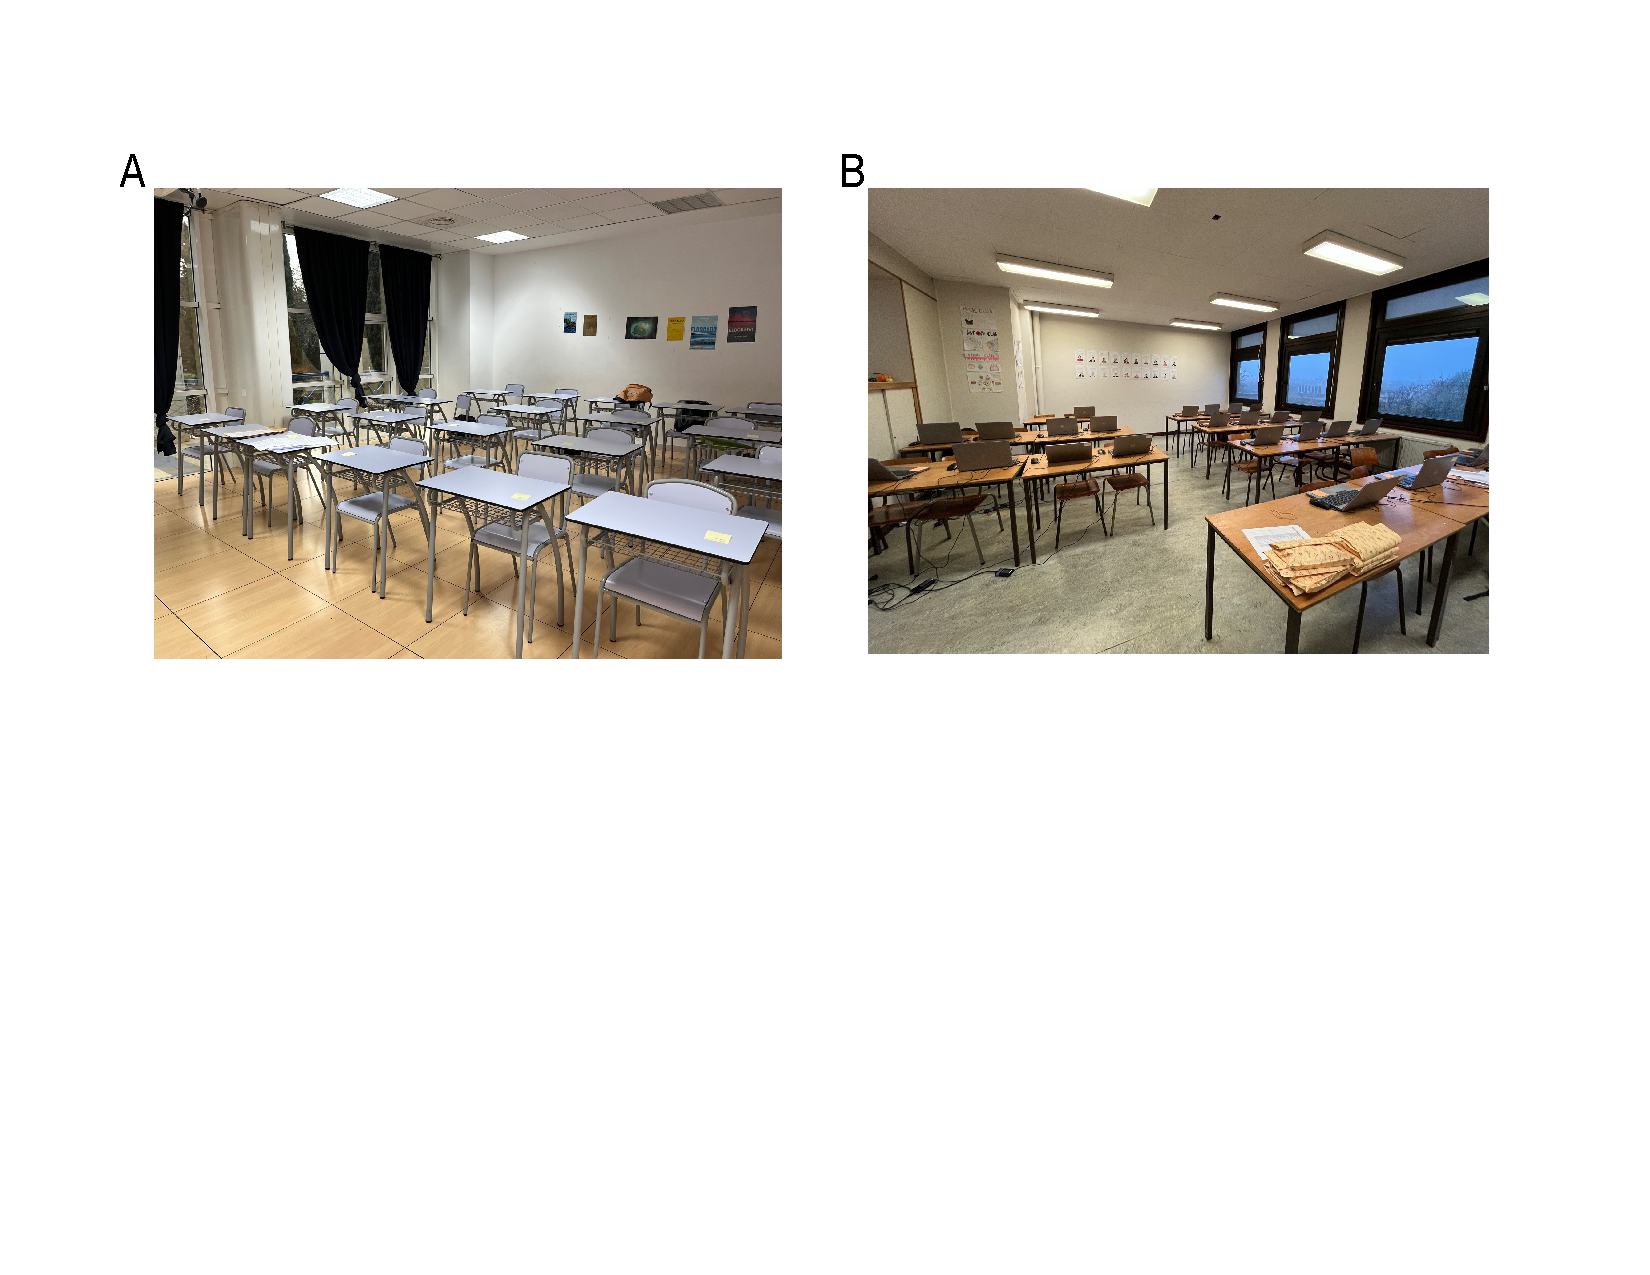
\includegraphics[keepaspectratio]{assets/pictures/classrooms.pdf}}
\caption{\label{fig:classrooms}Classrooms used for the experiment in Seville (\textbf{A}) and in Brussels (\textbf{B}).}
\end{figure}

\subsection{Experimental sessions}\label{experimental-sessions}

About ten experimental sessions were conducted at the schools between November 11 and 12, 2023, in Brussels and February 8 and 9, 2024, in Seville. Each session took about two hours. In the first 45-60 minutes, students received a personal computer and were asked to perform three main tasks using the AI tutor and answer a questionnaire without the AI tutor. In the following 45-60, there was a group discussion on how the students judged the interactions with the AI tutor and a more general debate on how they perceived the potential benefits and drawbacks of integrating LLMs in the classroom. The results of the group discussions are not discussed in this paper; however, they were used as material for interpreting the results of the experimental study.

\subsection{Experimental Conditions}\label{experimental-conditions}

Figure \ref{fig:design} illustrates the two randomised manipulations in our experimental design: (1) AI step-by-step reasoning and (2) Socratic vs non-Socratic AI. It is important to note that these were conducted as independent experiments, with different dependent and independent variables, rather than a factorial 2x2 design.

\begin{figure}
\centering
\pandocbounded{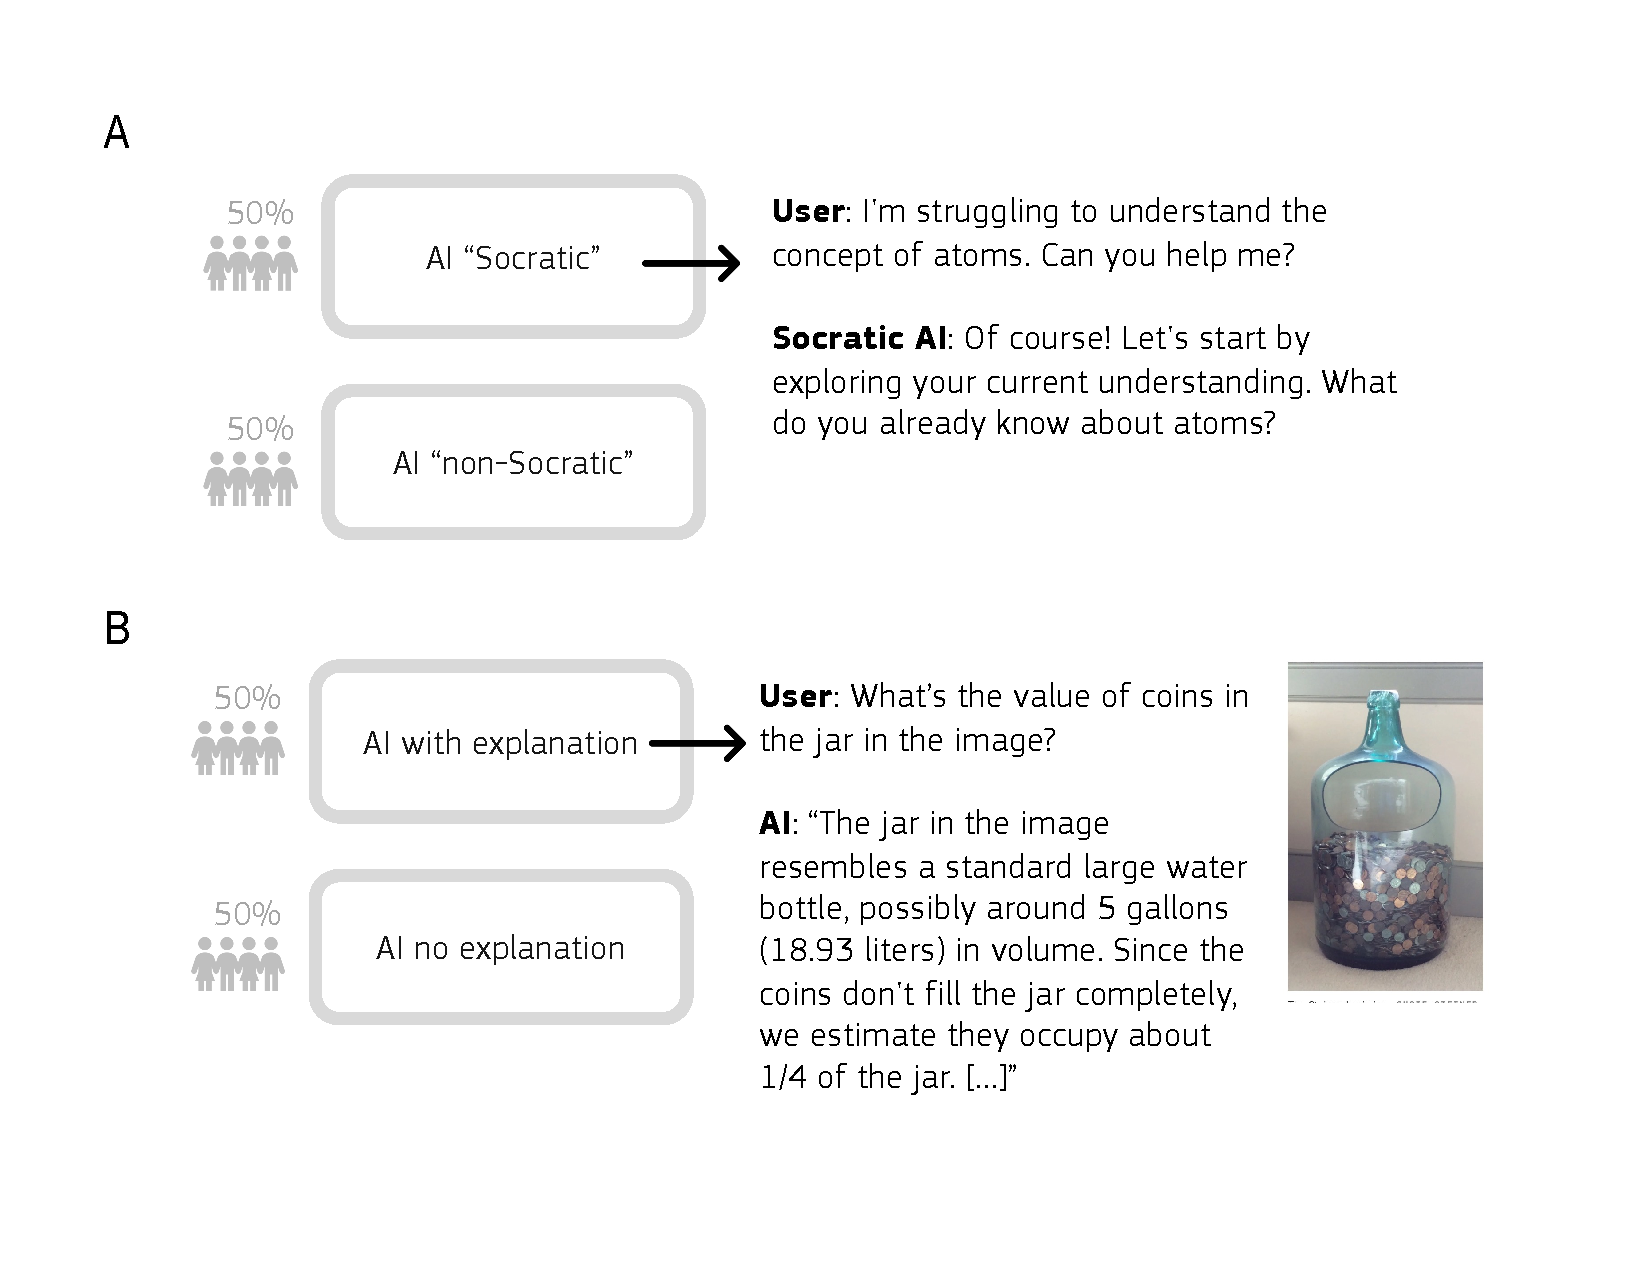
\includegraphics[keepaspectratio]{assets/pictures/experimental_design.pdf}}
\caption{\label{fig:design}The experimental design involves two manipulations: \textbf{A.} Socratic vs Non-Socratic; \textbf{B.} AI solution with explanation vs AI solution (without explanation)}
\end{figure}

\subsubsection{AI step-by-step reasoning}\label{ai-step-by-step-reasoning}

The first manipulation focuses on a task in which students are asked to estimate the value of coins in a jar (see Section \ref{sec:si-ai-explanation} for the details).\footnote{This is a common experimental activity in economics, especially in the context of auction theory (\citeproc{ref-thaler1988anomalies}{Thaler 1988}). The task is ideal in our setting because it requires participants to guess based on limited information, thus creating a situation where AI-generated assistance could potentially influence their decisions.} Specifically, we used the coin jar from Steiner's experiment (\citeproc{ref-steiner2015turns}{Steiner 2015}), aimed originally at assessing Internet users' guessing accuracy. For this intervention, we varied the AI's response by providing either a complete answer, which included both an estimated value and a step-by-step explanation generated by the AI tutor, or a partial answer that provided only the estimate without additional details. In both conditions, all participants received the same estimated value (\$213), but those in the full-answer condition also viewed an explanation outlining the step-by-step reasoning the AI used to arrive at this estimation based on the jar image.\footnote{Using GPT 4.0, we uploaded the image of the coin jar asking for an estimate of the value of coins ten times. We then selected the median response for the experiment.}

This setup allows us to examine how AI-provided explanations affect students' performance and their perceptions of the AI's accuracy. Specifically, we focus on three outcome variables: (1) the propensity to update their initial guess, (2) the accuracy of students' final estimations, measured as the (absolute) difference between their final guesses and the actual coin value, and (3) students' perceived accuracy of the AI, rated on a scale from low to high. We also asked participants (4) to rate the perceived accuracy of the mean guess among 600 people (\$596), which exaggerated the correct value, as reported in the original article (\citeproc{ref-steiner2015turns}{Steiner 2015}).

\subsubsection{Socratic vs Non-Socratic AI}\label{socratic-vs-non-socratic-ai}

The second manipulation involved randomly assigning students to one of two different types of AI tutors: Socratic or non-Socratic AI tutors. Both tutors were powered by the same underlying large language model (GPT-4). Still, each was instructed with different ``system messages'' to create different behaviours, as illustrated in Table \ref{tab:prompts}.\footnote{An AI's system message guides how the AI interprets the conversations by setting parameters for interaction.} For the Socratic tutor, the system message asked the model to engage students with open-ended, thought-provoking questions, encouraging them to think critically about their responses. In contrast, the non-Socratic AI tutor was instructed to provide concise, direct answers without necessarily engaging in deeper dialogue or posing further questions.

\begin{table}

\caption{\label{tab:prompts}Prompt instructions associated with the AI Tutor's treatments}
\centering
\begin{tabular}[t]{l>{\raggedright\arraybackslash}p{4in}}
\toprule
AI.Tutor & Prompt.instruction\\
\midrule
Socratic & You are a Socratic tutor. You always answer using the Socratic style, asking just the right questions to help students learn to think for themselves and breaking down the problem into simpler parts until it's at the right level for them. You provide concise information and explanations understandable for 8th to 10th grade students.\\
Non-Socratic & You are a didactic tutor. You provide concise information and explanations understandable for 8th to 10th grade students.\\
\bottomrule
\end{tabular}
\end{table}

This setup allows us to investigate the impact of different pedagogical AI tutoring approaches on students' performance and perceptions. Specifically, we asked students to use the AI tutor while performing three tasks: guess an unknown quantity (``How much water in litres do students consume at our school each week?''), express an opinion and write a short essay (``What is your opinion about the effect of social media on teenagers?''); respond to physics questions on how sound propagates in different media (``In which of the following materials does sound travel faster?''). These questions enabled us to assess the AI tutor's impact on students' learning and problem-solving abilities.

We focused on two primary metrics: (1) confidence in their answers and (2) perceived usefulness of interacting with the AI tutor. Specifically, students were asked, ``How confident are you that the answer you provided is accurate?'' on a five-point scale ranging from ``not confident at all'' to ``very confident.'' They were also asked, ``How helpful was it to interact with the AI tutor?'' This was also rated on a five-point scale, from ``Not at all helpful'' to ``Very helpful.'' Only for task 3, we had an additional metric, which was the correctness of their answers.

\subsection{Student Characteristics}\label{student-characteristics}

To examine student interactions with AI and their potential impact on learning and critical thinking, we collected a range of self-reported and behavioural data. The full questionnaire is provided in the Appendix (Section \ref{sec:questionnaire}).

\subsubsection{AI Attitudes and Usage}\label{ai-attitudes-and-usage}

To better understand students' general attitudes toward AI, we selected four questions from Schepman and Rodway's AI Attitudes Scale (\citeproc{ref-schepman2020initial}{Schepman and Rodway 2020}). These questions explored students; beliefs about AI's societal benefits, potential dangers, capacity to support learning, and the likelihood of misuse by students (Appendix, Section \ref{sec:questionnaire}). We also asked students about their direct experience using ChatGPT for homework --- the most common chatbot at the time of the study --- and their beliefs about how many of their peers use ChatGPT for their homework, thereby capturing both individual behaviour and the perceived social norm around AI usage. These measures help establish baseline orientations that may moderate how students engage with and evaluate AI explanations (related to RQ-1) and how they perceive different AI interaction styles (related to RQ-3).

\subsubsection{AI Academic Habits and Skills}\label{ai-academic-habits-and-skills}

Academic skills or habits may moderate the effect of AI interactions on problem-solving activities. Accordingly, to account for participants' heterogeneity in academic skills, we asked students to report their average school grades within five categories. We also asked students about their academic habits or the challenges they face at school, such as how often they complete their homework assignments on time and what factors affect their ability to do so.

\subsubsection{Student-AI Interaction Metrics}\label{student-ai-interaction-metrics}

To quantify engagement, we analyzed students' interaction logs with the AI Tutor, recording the number of turns and the word counts as a proxy for interaction intensity. While this provides a basic behavioural metric, it does not capture the quality of cognitive engagement or helpfulness, limiting its direct relevance to RQ-1 and RQ-2. Therefore, we also asked students about how useful they found the AI interactions and how confident they were in their answers to selected tasks. These self-reported metrics are needed to assess whether explanations were helpful to students (for RQ-1) and whether Socratic dialogue promoted critical thinking or confidence (for RQ-2).

\section{Results}\label{sec:results}

\subsection{Overview of Student Demographics}\label{overview-of-student-demographics}

A total of 122 students participated in the study, 64 in Brussels and 58 in Seville. The sample was gender balanced. Over half of the students reported B+ grades and prior use of ChatGPT, with boys more likely to report ChatGPT experience. Around 50\% reported to always complete homework on time, with a minority reporting less than always, with factors like time management (17\% in Brussels, 25\% in Seville) and material comprehension (56\% in Brussels, 28\% in Seville) affecting completion. Students' self-efficacy varied by task, with 30\% of the students feeling they could ``easily'' write a technology essay (task 2) but only 6\% and 11\% feeling confident about explaining sound propagation (task 3) or solving a numerical estimation task such as guessing the litres of water in a pool (task 1). Thus, the sample was substantially homogeneous in terms of demographics but diverse in terms of self-efficacy.

Table \ref{tab:summary-statistics} illustrates the distribution of student characteristics across treatment groups alongside the results of separate Fisher's Exact Tests on the association with treatment assignment. The sample characteristics were generally balanced across treatment groups. Only one variable out of ten -- i.e., self-reported difficulties in homework -- was statistically associated (p = 0.05) with the Socratic/Non-Socratic assignment, while no significant associations were found for the AI-reasoning assignment. Thus, only one out of twenty Fisher's exact tests showed a significant result, indicating a good balance across treatments.

\begin{table}
\centering
\caption{\label{tab:summary-statistics}Sample Characteristics}
\centering
\begin{tabular}[t]{llrrlrrlr}
\toprule
\multicolumn{2}{c}{ } & \multicolumn{3}{c}{Socratic (\%)} & \multicolumn{3}{c}{AI Explain (\%)} & \multicolumn{1}{c}{ } \\
\cmidrule(l{3pt}r{3pt}){3-5} \cmidrule(l{3pt}r{3pt}){6-8}
Name & Value & Yes & No & p. & Yes & No & p. & N\\
\midrule\arrayrulecolor{gray!20}
Gender & Boy & 55 & 47 & 0.47 & 49 & 53 & 0.72 & 62\\
\hline
 & Girl & 45 & 53 &  & 51 & 47 &  & 59\\
\hline
Grades & Average or lower grades & 47 & 45 & 0.86 & 43 & 48 & 0.58 & 55\\
\hline
 & Top grades & 53 & 55 &  & 57 & 52 &  & 65\\
\hline
Has used ChatGPT & No & 43 & 37 & 0.58 & 34 & 45 & 0.27 & 49\\
\hline
 & Yes & 57 & 63 &  & 66 & 55 &  & 73\\
\hline
Homework difficulties & Clear instructions from teachers & 10 & 20 & 0.05 & 14 & 16 & 0.53 & 18\\
\hline
 & Effective time management & 29 & 12 &  & 25 & 17 &  & 25\\
\hline
 & Lack of distractions & 18 & 10 &  & 9 & 19 &  & 17\\
\hline
 & Support from family or peers & 8 & 7 &  & 9 & 6 &  & 9\\
\hline
 & Understanding the material & 35 & 51 &  & 44 & 42 &  & 52\\
\hline
Homework on time & Always on time & 42 & 56 & 0.33 & 56 & 42 & 0.27 & 59\\
\hline
 & Sometimes or rarely on time & 8 & 7 &  & 5 & 9 &  & 9\\
\hline
 & Usually on time & 50 & 37 &  & 39 & 48 &  & 53\\
\hline
Homework weekly study & 0-1 hours & 47 & 41 & 0.52 & 44 & 44 & 0.12 & 53\\
\hline
 & 1-2 hours & 34 & 44 &  & 46 & 33 &  & 47\\
\hline
 & 2+ hours & 19 & 15 &  & 11 & 23 &  & 21\\
\hline
Location & Brussels & 49 & 56 & 0.47 & 50 & 55 & 0.72 & 64\\
\hline
 & Seville & 51 & 44 &  & 50 & 45 &  & 58\\
\hline
Self-efficacy (essay) & Could do easily & 38 & 32 & 0.73 & 29 & 41 & 0.45 & 43\\
\hline
 & Could do with a bit of effort & 52 & 53 &  & 55 & 50 &  & 64\\
\hline
 & I couldn't do this on my own & 3 & 3 &  & 5 & 2 &  & 4\\
\hline
 & I would struggle on my own & 6 & 12 &  & 10 & 8 &  & 11\\
\hline
Self-efficacy (guess) & Could do easily & 14 & 12 & 0.60 & 9 & 17 & 0.17 & 16\\
\hline
 & Could do with a bit of effort & 27 & 34 &  & 36 & 25 &  & 37\\
\hline
 & I couldn't do this on my own & 24 & 15 &  & 24 & 16 &  & 24\\
\hline
 & I would struggle on my own & 35 & 39 &  & 31 & 42 &  & 45\\
\hline
Self-efficacy (sound) & Could do easily & 6 & 7 & 0.35 & 7 & 6 & 0.66 & 8\\
\hline
 & Could do with a bit of effort & 46 & 31 &  & 33 & 44 &  & 47\\
\hline
 & I couldn't do this on my own & 14 & 17 &  & 17 & 14 &  & 19\\
\hline
 & I would struggle on my own & 33 & 46 &  & 43 & 36 &  & 48\\
\arrayrulecolor{black}\bottomrule
\end{tabular}
\end{table}

\subsection{Attitudes Towards AI}\label{attitudes-towards-ai}

As illustrated in Figure \ref{fig:attitudes-AI}, students expressed conflicting views on the role of AI in education. On the one hand, a majority felt that AI is often misused by students (65\%) and potentially dangerous (57\%). On the other hand, most students also anticipated that AI would enhance student learning in the future (59\%) and contribute positively to society (65\%). These findings suggest that most students in our sample are aware of the risks of misuse and safety with a prevailing optimism that AI could support educational growth and societal progress.

\begin{figure}
\centering
\pandocbounded{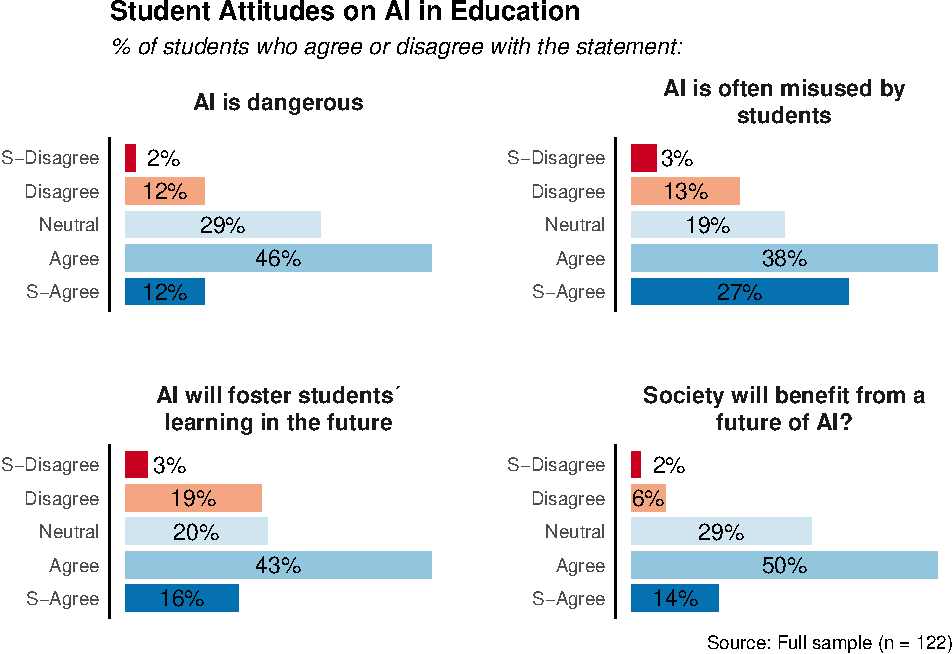
\includegraphics[keepaspectratio]{HSSC_Revised_Submission/main_report_files/figure-latex/attitudes-AI-1.pdf}}
\caption{\label{fig:attitudes-AI}Student attitudes on AI in education}
\end{figure}

\subsection{The Impact of AI Step-by-step Reasoning Exposure}\label{the-impact-of-ai-step-by-step-reasoning-exposure}

Nearly all students revised their initial estimates (110 out of 122), with no significant difference between treatment groups (Fisher's test, p = 0.9). However, presenting students with AI-generated step-by-step reasoning may have influenced the accuracy of their revised estimates.

To address RQ1, we examined whether the treatment---showing step-by-step AI reasoning---affected how students used the AI's prediction, compared to seeing the prediction alone without any accompanying explanation. For each student \(i = 1, \cdots, 122\), we computed the absolute error as the absolute difference between student \(i\)'s guess, \(\text{Guess}_i\), and the actual value of coins:
\[
  \text{Absolute Error}_i = \mid \text{Guess}_i - \text{Actual Value Coins} \mid,
\]
where a smaller absolute error indicated greater accuracy.

Figure \ref{fig:boot-accuracy} illustrates that students' prediction accuracy was positively skewed in both treatment groups, with a greater accuracy for students exposed to AI reasoning. To estimate confidence intervals for the median difference in accuracy betweeen the groups, we used a nonparametric bootstrap approach.\footnote{We detected one outlier in the data, which was removed from the bootstrap analysis: one student provided an unusual and notably high guess of 6969. However, this value deviated substantially from both the overall distribution and the student's initial guess, suggesting a mistake rather than an estimate.} This procedure involved resampling participants' absolute errors (n = 1,999) to build a distribution of medians for each group. The 5th and 95th percentiles of the resulting distribution were used to construct a 90\% confidence interval for the difference in accuracy between groups. The interval ranged from 0 to 70, indicating a greater accuracy (lower error) for the students exposed to AI-generated reasoning (one-sided, p \textless{} 0.05).

\begin{figure}
\centering
\pandocbounded{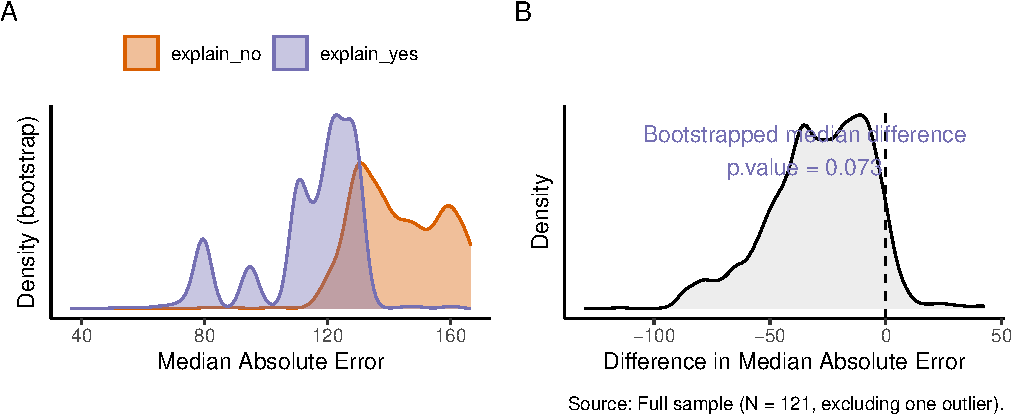
\includegraphics[keepaspectratio]{HSSC_Revised_Submission/main_report_files/figure-latex/boot-accuracy-1.pdf}}
\caption{\label{fig:boot-accuracy}Comparison of Students' Absolute Error in Estimating Coin Jar Value with and without AI Explanations. All students received the AI-generated estimate of \$213 (the correct value was \$379.54). Still, those in the AI reasoning treatment also viewed the AI-generated step-by-step explanation for the estimation. Exposure to the AI-generated explanation significantly reduced the students' median absolute error.}
\end{figure}

To examine the impact of AI explanations on students' perceived credibility of AI predictions (RQ2), we analysed students' five-point ratings of the perceived accuracy of the AI estimated value of coins. We noticed that 53\% of students who did not receive step-by-step reasoning considered the AI estimate as either ``good'' (39\%) or ``very good'' (14\%) compared to 43\% of students exposed to the AI reasoning (19\% and 24\%, respectively). This gap of ten percentage points suggests that students viewed the AI as more accurate when the AI-generated guess was presented as a ``black box.'' However, we didn't have enough observations to reach a statistically significant association (Fisher's test, p = .27), and even regression analysis, controlling for individual characteristics, showed no significant association (Figure \ref{fig:perceived-accuracy-coins}).

Conversely, exposure to the AI step-by-step reasoning seemed associated with students' perception of the accuracy of the ``human'' guess --- the average guess from 600 participants reported in the original study (\citeproc{ref-steiner2015turns}{Steiner 2015}).\footnote{Notably, this guess was \$596, exceeding the correct value (\$379.54) by about the same amount as the AI guess underestimated it (\$213).} While all groups received the same human and AI estimates, 64\% of students in the control rated the human estimate as ``poor'' or ``very poor'' against 45\% of students exposed to AI reasoning. Although this difference was insignificant (Fisher's exact test, p = 0.15), regression analysis, controlling for fixed differences across schools and across individuals, such as their gender, the initial guess of the value of coins, and experience with ChatGPT, showed a significant effect (p \textless{} 0.05) of the assignment to AI reasoning on students' perceptions of the human guess, as shown in Figure \ref{fig:perceived-accuracy-coins}. This finding underscores the complex relationship between AI and learning. It suggests that students exposed to the AI's step-by-step reasoning may have identified minor errors, thus increasing their expectations of human accuracy, and those who viewed AI as a ``black box'' tended to underrate human estimates.

\begin{figure}
\centering
\pandocbounded{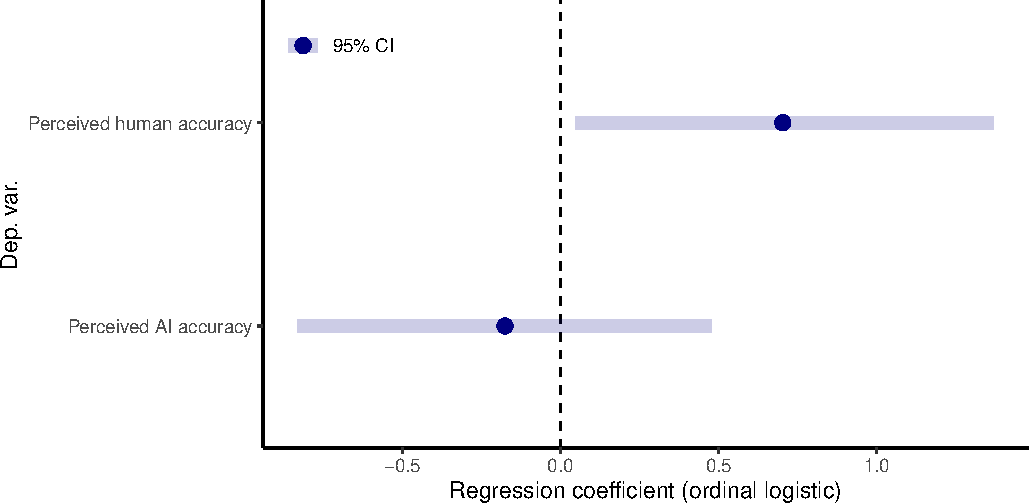
\includegraphics[keepaspectratio]{HSSC_Revised_Submission/main_report_files/figure-latex/perceived-accuracy-coins-1.pdf}}
\caption{\label{fig:perceived-accuracy-coins}Comparison of students' perceived accuracy of AI and human estimates across treatments on a five-point scale. Coefficients from separate ordinal logistic regressions controlling for students' location, gender, and prior experience with ChatGPT. Positive coefficients indicate increased perceived accuracy associated with students' exposure to AI reasoning.}
\end{figure}

\subsection{A Comparison of Socratic vs Non-Socratic AI}\label{a-comparison-of-socratic-vs-non-socratic-ai}

\subsubsection{Student-AI Interactions}\label{student-ai-interactions}

Figure \ref{fig:messages} shows the students' message length and frequency in the Socratic AI and Non-Socratic AI groups, allowing us to compare the student-AI interactions across treatment groups. As shown in the figure, Socratic AI students exchanged a median of 20 messages, significantly more than the eight messages by non-Socratic AI students (Wilcoxon test, p \textless{} 0.01). In addition, the Socratic AI's messages were significantly shorter, with a median of 42 words, compared to 123 for the non-Socratic tutor (Wilcoxon test, p \textless{} 0.01). Socratic students also used fewer words, with two peaks: one at ten and the other at one word. This evidence supports the hypothesis that the Socratic tutor encouraged more engagement and interaction, resembling a relatively more genuine student-tutor talk.

\begin{figure}
\centering
\pandocbounded{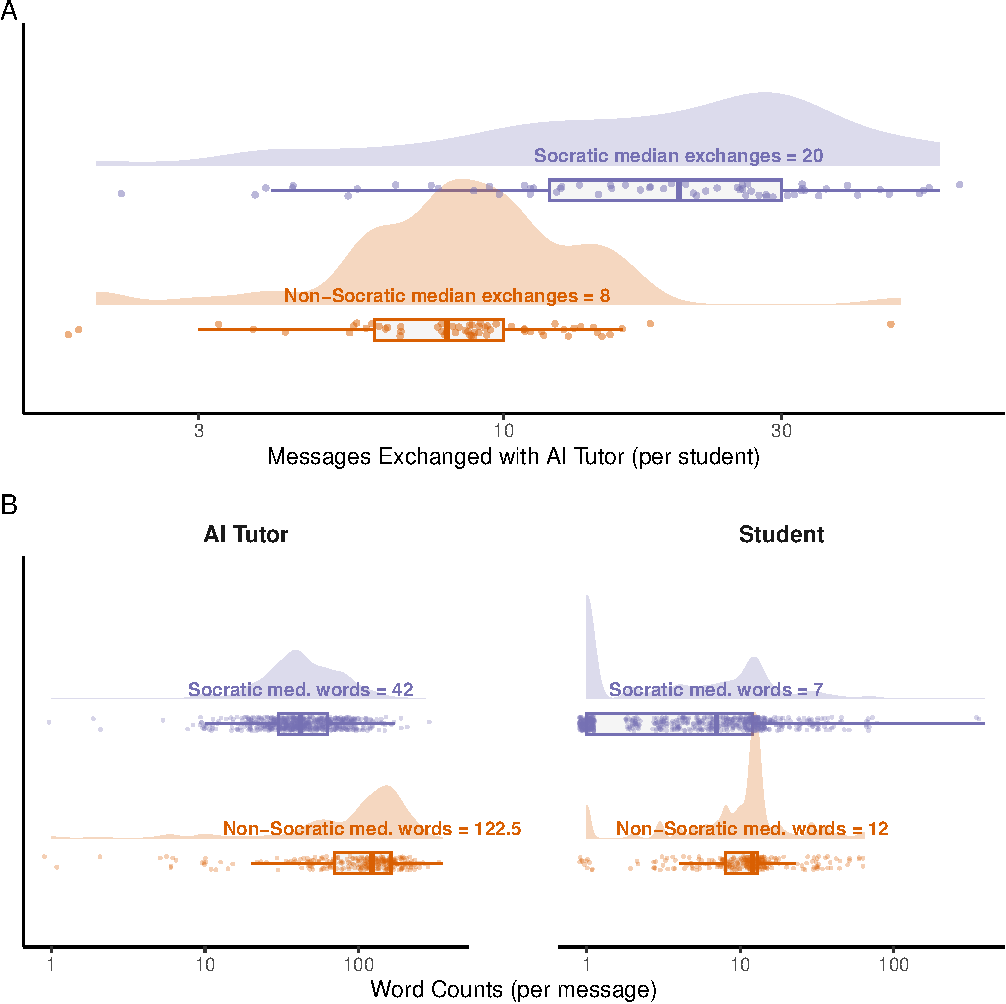
\includegraphics[keepaspectratio]{HSSC_Revised_Submission/main_report_files/figure-latex/messages-1.pdf}}
\caption{\label{fig:messages}Comparison of message frequency and word count per message across Socratic and non-Socratic treatments. Top panel (\textbf{A}) shows differences in the frequency of messages exchanged, while the bottom panels (\textbf{B} ) depict the word counts per message for the AI tutor (left) and the students (right).}
\end{figure}

\subsubsection{Students' Confidence in Their Responses}\label{students-confidence-in-their-responses}

To test whether Socratic AI increased students' confidence in their answers (RQ4), we examined students' self-reported confidence levels at the end of each task. As shown in Figure \ref{fig:confidence}, the observed differences in confidence between the treatment groups were minimal. Specifically, 25\% of Socratic students reported feeling ``very confident,'' and 33\% reported feeling ``confident'' compared to 21\% and 38\%, respectively, among non-Socratic students. These differences were not statistically significant, even with regression analysis controlling for variation across students and tasks (Figure \ref{fig:confidence-regression}). Thus, our analysis found no evidence of treatment effects on students' confidence in their answers.

\begin{figure}
\centering
\pandocbounded{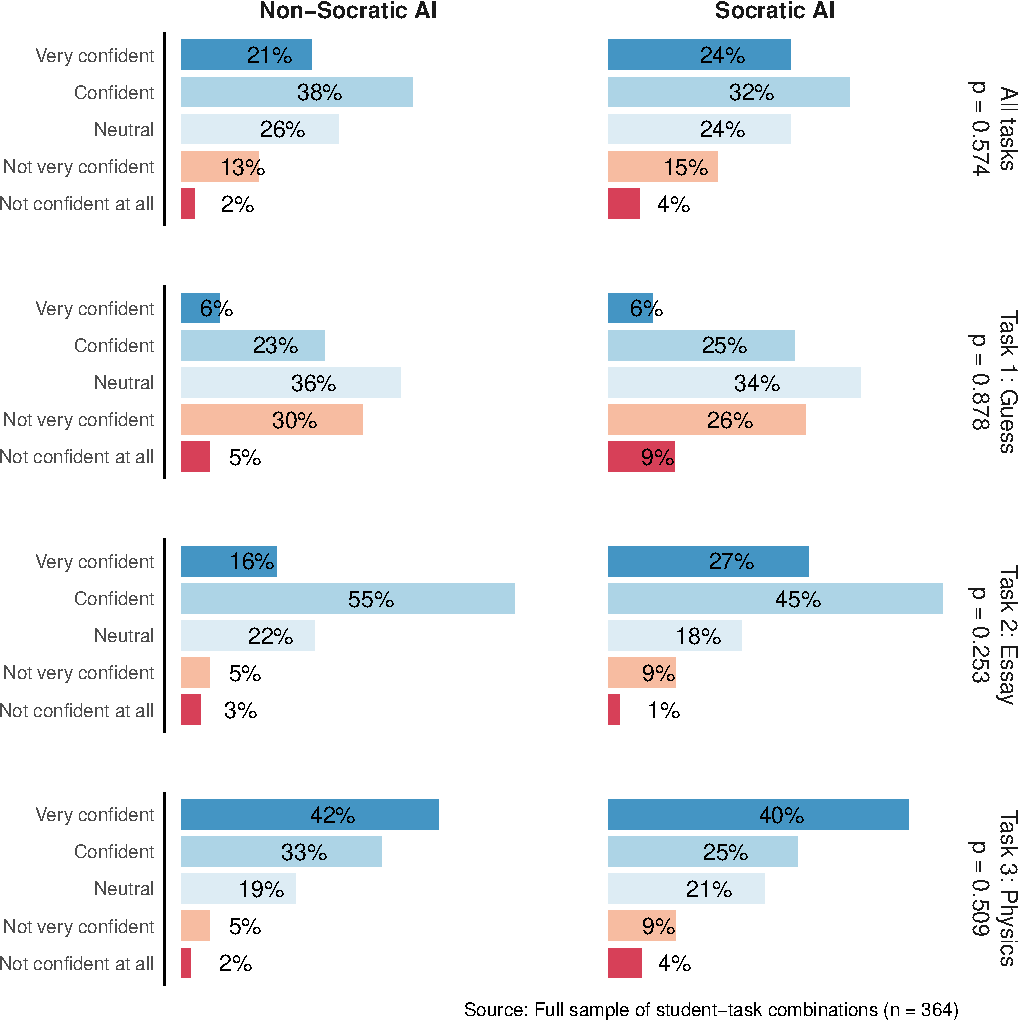
\includegraphics[keepaspectratio]{HSSC_Revised_Submission/main_report_files/figure-latex/confidence-1.pdf}}
\caption{\label{fig:confidence}This figure shows the impact of Socratic AI on students' confidence levels in their performance across three different tasks. Despite some differences between the Socratic and Non-Socratic groups, we found no significant association between the treatment assignment and students' declared confidence levels.}
\end{figure}

\begin{figure}
\centering
\pandocbounded{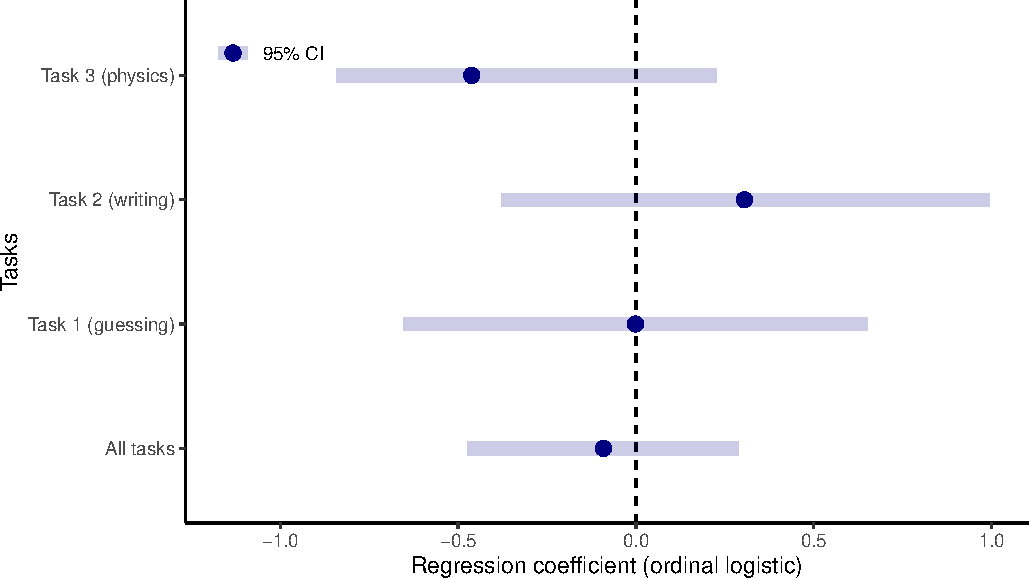
\includegraphics[keepaspectratio]{HSSC_Revised_Submission/main_report_files/figure-latex/confidence-regression-1.pdf}}
\caption{\label{fig:confidence-regression}This figure shows the coefficients from separate ordinal logistic regressions on students' confidence in their answer on a five-point scale, controlling for students' self-efficacy per task and task fixed effect. Results show no significant association between the treatment assignment and students' confidence levels.}
\end{figure}

Further explorative regression analysis to examine potential treatment interactions shows that Socratic AI students with prior ChatGPT experience reported significantly less confidence (p \textless{} 0.1) than Non-Socratic AI students (see Figure \ref{fig:interactions}). This explorative finding suggests that experienced users may perceive new or unconventional AI tutoring methods as less effective or even counterproductive, indicating that encouraging the use of such AI tutoring tools among experienced ChatGPT students can be challenging.

\subsubsection{Perceived Helpfulness of AI Tutor}\label{perceived-helpfulness-of-ai-tutor}

To test differences in students' perceptions of the AI tutor's helpfulness (RQ5), we examined students' ratings of helpfulness of the AI interaction at the end of each task. These ratings were on a five-point scale, from ``Not at all helpful'' to ``Very helpful.''\footnote{Due to a coding issue, the scale used in Brussels and Seville differed slightly in the labels: Seville's students saw ``Extremely helpful'' whereas Brussels students saw ``Very helpful.'' However, this issue has a minimal impact on the overall results, as results focus on the negative labels (``not at all helpful'' or ``not helpful'') and they remain the same even after controlling for location effects in a regression. Additionally, open discussions held with students after the experimental session confirmed that they found the Socratic AI less helpful. This feedback, combined with the observed differences in negative labels, reinforces that the coding discrepancy has a minimal impact on the overall findings.}

In both treatment groups, many students found interacting with the AI tutor ``very helpful'' or ``helpful'', with 56\% of the non-Socratic and 44\% of the Socratic students, as shown in Figure \ref{fig:helpfulness}. However, the Socratic treatment group showed a bimodal distribution, with a substantial fraction of students (21\%) finding the interaction ``not at all helpful.'' The association between perceived helpfulness and treatment assignment was statistically significant (Fisher's exact test, p = 0.025), providing evidence that Socratic AI was less helpful to certain students. This association, however, was stronger for Task 1 and Taks 3 than Task 2, suggesting an association between the perceived AI's helpfulness and the type of task. Ordinal logistic regression accounting for individual student and task characteristics, including self-efficacy per task, revealed a statistically significant negative difference that corresponds to a drop of approximately 13 percentage points in perceived helpfulness associated with the Socratic AI, as illustrated in Figure \ref{fig:helpful-regression}. See Section \ref{sec:regress-confidence} for more details.

\begin{figure}
\centering
\pandocbounded{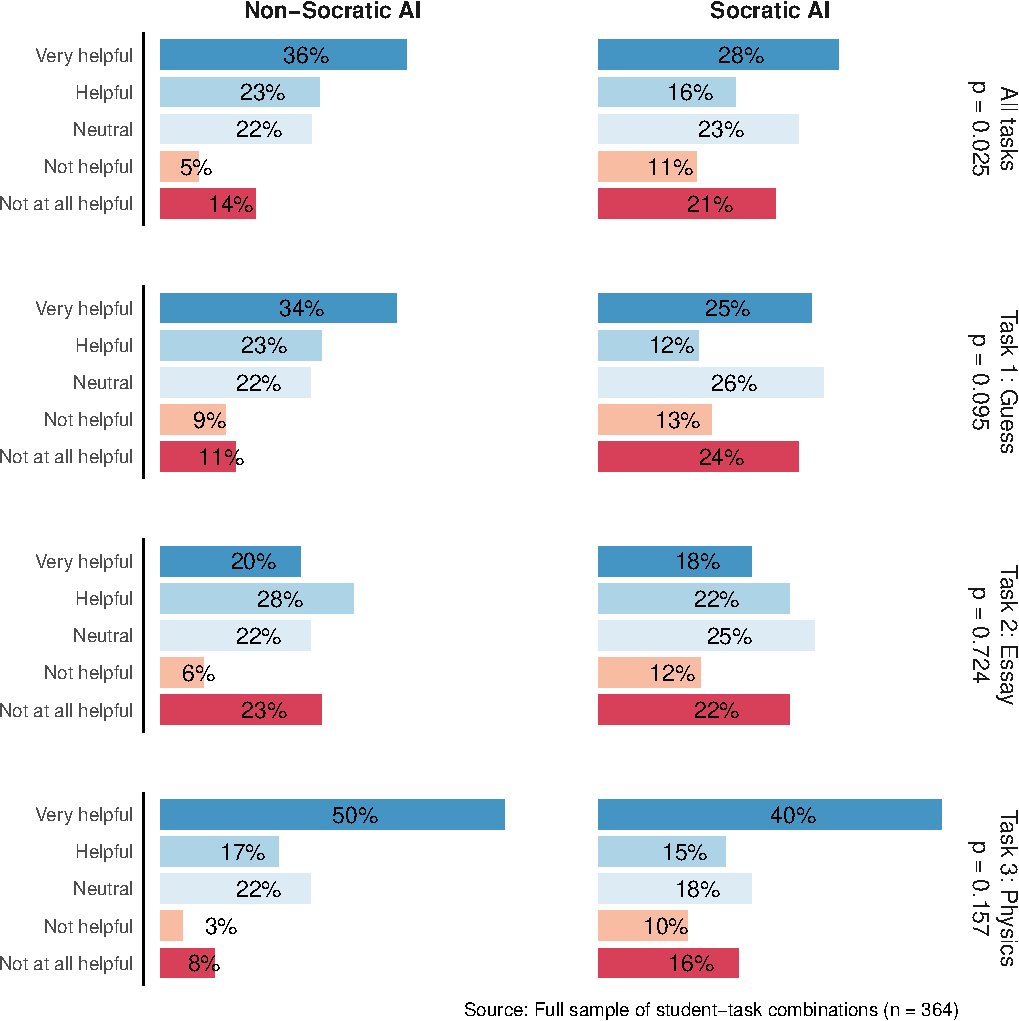
\includegraphics[keepaspectratio]{HSSC_Revised_Submission/main_report_files/figure-latex/helpfulness-1.pdf}}
\caption{\label{fig:helpfulness}This figure shows the impact of Socratic AI on students' perceived helpfulness of the AI tutor across three different tasks.}
\end{figure}

\begin{figure}
\centering
\pandocbounded{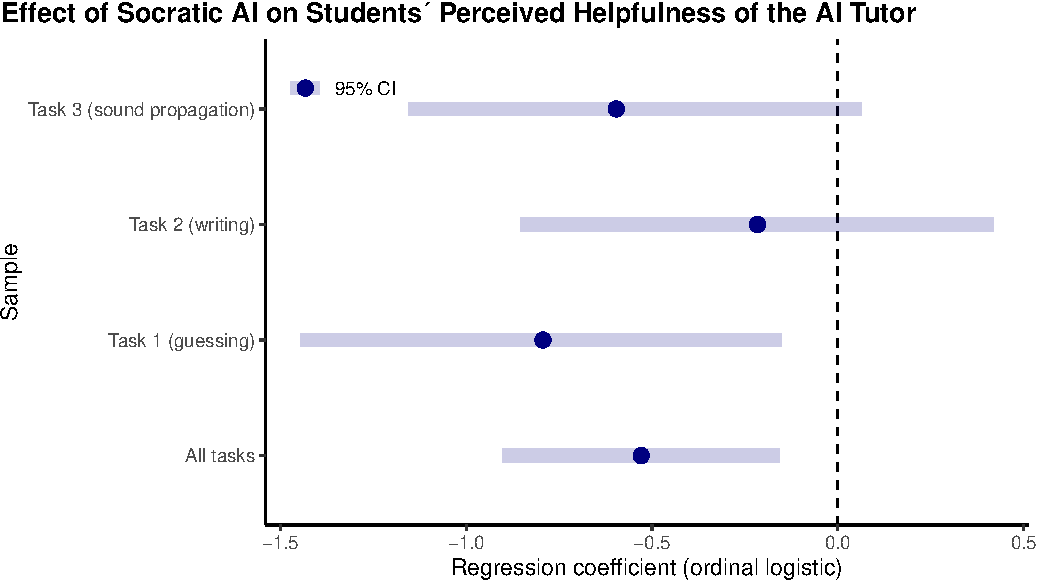
\includegraphics[keepaspectratio]{HSSC_Revised_Submission/main_report_files/figure-latex/helpful-regression-1.pdf}}
\caption{\label{fig:helpful-regression}The impact of Socratic AI on students' confidence levels in their performance across three different tasks. Despite some differences between the Socratic and Non-Socratic groups, we found no significant association between the treatment assignment and students' declared confidence levels}
\end{figure}

\subsubsection{Learning Outcomes and Knowledge Retention}\label{learning-outcomes-and-knowledge-retention}

To evaluate the impact of learning (RQ3), we compared the correctness of responses to Task 3, which focused on sound propagation, and assessed knowledge retention using a follow-up question on the same topic without AI assistance. As shown in Figure \ref{fig:learning}, the use of AI significantly enhanced students' response accuracy. Before interacting with the AI tutor, only 32\% of students correctly answered that sound travels faster in water than air due to water's higher density. After AI interaction, this percentage nearly doubled increasing to 68\%. However, there was no significant difference in learning outcomes between the Socratic and non-Socratic AI approaches, as illustrated in the figure. Moreover, when presented with a follow-up question (asking in which medium sound travels fastest among gold, rubber, warm air, cold air, and water), only 18\% of students responded correctly by selecting the denser material (i.e., gold), again with no significant difference across treatments. This result suggests two implications. Firstly, we found no evidence of Socratic AI improving learning. Secondly, our results seems to suggest a problem of limited retention of the insights obtained with AI assistance or difficulty in applying such learning to novel scenarios.\footnote{While it is true that gold is significantly denser than water or air, it is possible that some students did not fully understand this fact or were unsure how to compare the densities of the materials. If that were the case, even if the AI effectively conveyed that sound travels faster in denser media, students lacking this knowledge may still have been unable to select the correct answer. However, this explanation seems unlikely, as the relative densities of air, water, and metals, like gold, are commonly taught and conceptually straightforward, suggesting that other factors have contributed to students' outcomes.}

\begin{longtable}[]{@{}
  >{\raggedright\arraybackslash}p{(\linewidth - 6\tabcolsep) * \real{0.5698}}
  >{\raggedleft\arraybackslash}p{(\linewidth - 6\tabcolsep) * \real{0.1395}}
  >{\raggedleft\arraybackslash}p{(\linewidth - 6\tabcolsep) * \real{0.1512}}
  >{\raggedleft\arraybackslash}p{(\linewidth - 6\tabcolsep) * \real{0.1395}}@{}}
\caption{\label{tab:learning}\% of students in each treatment group by responses to the question `Does sound travel faster in water than air?'}\tabularnewline
\toprule\noalign{}
\begin{minipage}[b]{\linewidth}\raggedright
\end{minipage} & \begin{minipage}[b]{\linewidth}\raggedleft
Full sample
\end{minipage} & \begin{minipage}[b]{\linewidth}\raggedleft
Non-Socratic
\end{minipage} & \begin{minipage}[b]{\linewidth}\raggedleft
Socratic AI
\end{minipage} \\
\midrule\noalign{}
\endfirsthead
\toprule\noalign{}
\begin{minipage}[b]{\linewidth}\raggedright
\end{minipage} & \begin{minipage}[b]{\linewidth}\raggedleft
Full sample
\end{minipage} & \begin{minipage}[b]{\linewidth}\raggedleft
Non-Socratic
\end{minipage} & \begin{minipage}[b]{\linewidth}\raggedleft
Socratic AI
\end{minipage} \\
\midrule\noalign{}
\endhead
\bottomrule\noalign{}
\endlastfoot
Same speed & 9.1 & 6.8 & 11.3 \\
Water is faster because higher density (correct) & 31.4 & 35.6 & 27.4 \\
Water is faster because lower density & 11.6 & 10.2 & 12.9 \\
Water is slower because higher density & 41.3 & 42.4 & 40.3 \\
Water is slower because lower density & 6.6 & 5.1 & 8.1 \\
\end{longtable}

\begin{figure}
\centering
\pandocbounded{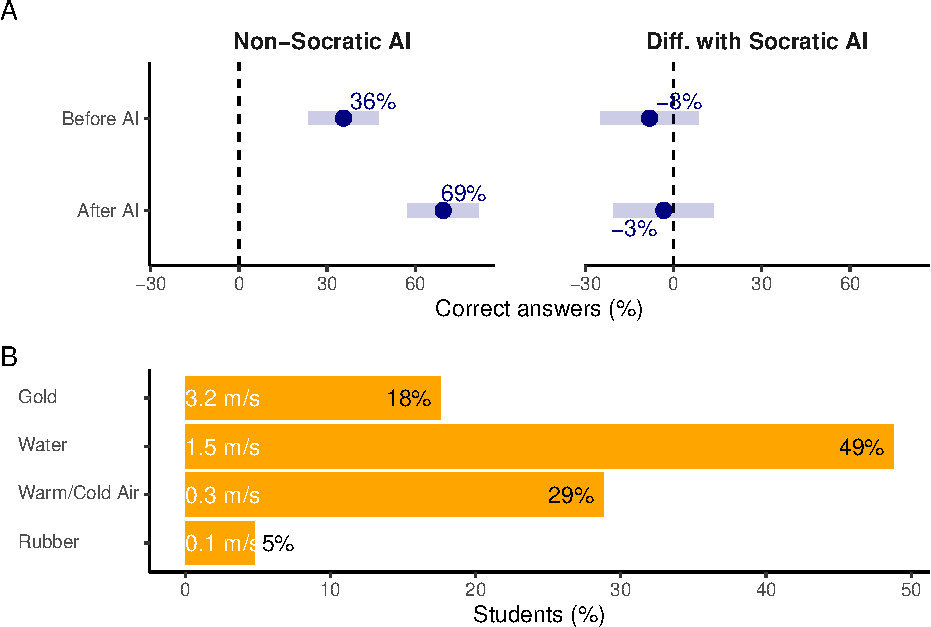
\includegraphics[keepaspectratio]{HSSC_Revised_Submission/main_report_files/figure-latex/learning-1.pdf}}
\caption{\label{fig:learning}Effects on learning: \textbf{A} shows the \% of correct responses about the physics of sound propagation, illustrating the positive effect of interacting with the AI tutor, while no differences are associated with the Socratic AI. \textbf{B} shows the results of the verification question asking students to identify the fastest material for sound propagation (speed as meter per second reported) without AI assistance. Only 18\% responded accurately, indicating limited learning.}
\end{figure}

\begin{figure}
\centering
\pandocbounded{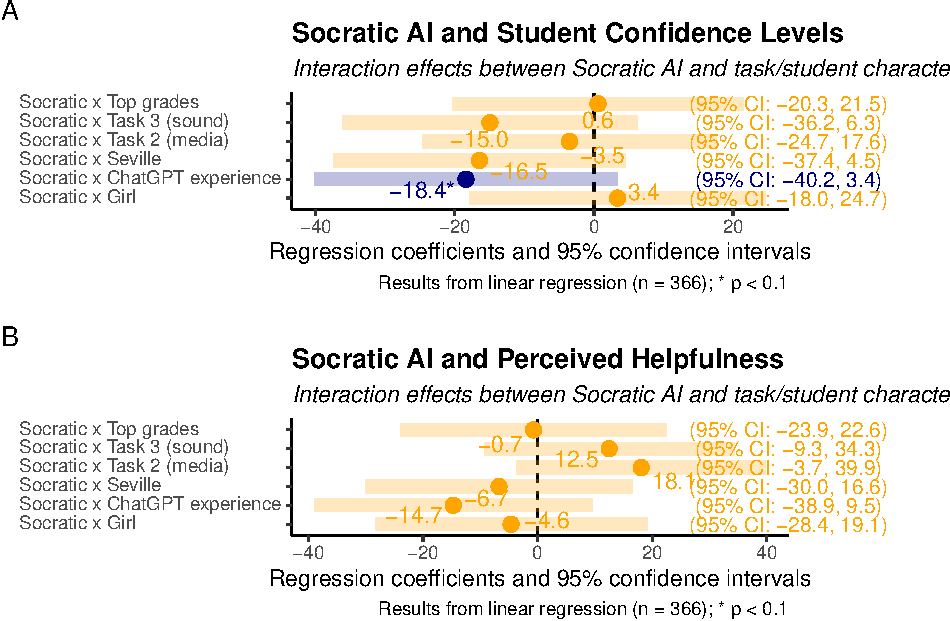
\includegraphics[keepaspectratio]{HSSC_Revised_Submission/main_report_files/figure-latex/interactions-1.pdf}}
\caption{\label{fig:interactions}Regression coefficients and 95\% confidence intervals from a linear regression using as dependent variable the (\textbf{A}) students' self-reported confidence level and (\textbf{B}) perceived helpfulness of the AI tutor. The controls include student's gender, grades, location, and ChatGPT experience. Treatment dummies are interacted with all the controls and the task type. All models also include individual student random effects, and the student's rated confidence in their skills before performing each task.}
\end{figure}

\section{Discussion}\label{discussion}

This study contributes to our understanding of the impact of pedagogically-aligned configurations of an LLM-based tool on the learning and attitudes of high school students, with a special focus on their critical thinking.

\subsection{Overview of the findings}\label{overview-of-the-findings}

With the rapid adoption of AI in education, the focus on students' competencies and skills, such as critical thinking, has become particularly urgent (\citeproc{ref-walter2024embracing}{Walter 2024}; \citeproc{ref-holmes2023guidance}{Holmes, Miao, et al. 2023}). Despite the rapidly increasing body of research on the impact of LLMs on students' learning, most studies focus on participants in higher education (e.g., \citeproc{ref-suriano2025student}{Suriano et al. 2025}), which may not generate insights applicable to younger students with different cognitive maturity. In addition, despite the increasing research interest regarding the impact of LLMs on students' learning, there is little consensus among researchers, mainly due to students' over-reliance on AI tools (\citeproc{ref-zhai2024effects}{Zhai, Wibowo, and Li 2024}).

The results of this study focus on the role of two interventions in configuring an LLM chatbot for educational support: (i) step-by-step explanations and (ii) the Socratic method with guiding questions. First, we found that students significantly benefit from AI-generated step-by-step reasoning accompanying solutions, mainly when performing open-ended tasks like estimating unknown quantities (RQ1). This finding aligns with expectations of current research on the use of LLM chatbots and their ability to provide explanations for learning purposes (\citeproc{ref-wu2024critical}{Y. Wu 2024}). It also aligns with previous research demonstrating that LLMs can enhance student performance (\citeproc{ref-xing2025development}{Xing et al. 2025}). However, our results underscore that the key mechanism driving AI improvements is the step-by-step reasoning provided by the AI, which allows students to understand better and engage with problem-solving.

Furthermore, our study reveals that step-by-step reasoning not only helps students in solving problems but also enhances students' ability to evaluate AI-generated information critically (RQ2). Critical thinking is indeed a complex cognitive process that involves the evaluation and analysis of a given information (\citeproc{ref-lai2011critical}{Lai 2011}). The mobilisation of students' critical thinking in the specific task was evidenced by the more positive evaluations of human-generated guesses compared to AI-generated solutions, suggesting that students could better assess and challenge AI predictions. This contribution extends the existing literature by showing that AI can foster critical thinking and analytical skills when coupled with transparent reasoning rather than being presented as a ``black box'' (\citeproc{ref-bearman2023learning}{Bearman and Ajjawi 2023}).

In addition, we compared various ways to structure student-AI interactions and, more specifically, the effectiveness of Socratic AI (an interactive, questioning-based AI) with non-Socratic AI. Our results showed that Socratic AI was more engaging and promoted greater interaction, aligning with the notion that AI-student interactions should be dynamic and dialogical (\citeproc{ref-suriano2025student}{Suriano et al. 2025}). However, contrary to our expectations, we found no significant differences in students' self-reported confidence in the accuracy of their answers or in the correctness of their responses despite the more frequent interactions with the Socratic AI (RQ4). Additionally, the Socratic AI's perceived helpfulness was rated lower compared to the non-Socratic AI (RQ5). These results cast some doubts on the effectiveness of Socratic AI in short-term tasks or, more broadly, the effect of certain kinds of AI-student interactions. As such, existing pedagogical practices extensively used in human-human interaction might not always work in human-AI interaction. In addition, while recent research attempts to understand the quality of Socratic LLMs for critical thinking (e.g., \citeproc{ref-favero2024enhancing}{Favero et al. 2024}), these studies use simulations without experiments with human participants. Our results underscore the need for adapting existing pedagogical paradigms or proposing new ones for integrating LLM tools into pedagogical practices effectively.

Interestingly, our findings indicate that simply interacting with AI cannot promote meaningful and lasting learning (RQ3). In our initial test on sound propagation, approximately half of the students could revise their initial answers based on AI interactions, improving their response accuracy from 30\% to 70\%. However, in a verification task where students had no access to AI, the majority failed to identify the correct answer, mistakenly claiming that sound propagates faster in water than in gold. Most students exhibited this misunderstanding, which supports key concerns that AI-generated answers alone do not scaffold effective learning and the mere implementation of Socratic AI does not mitigate this risk.

Our results suggest that AI has great potential as an educational tool, but its implementation requires careful consideration. First, students with prior experience in using AI tools may not readily adopt new pedagogical approaches, especially if they perceive them as less effective than commercially available alternatives. Second, the effectiveness of the pedagogical approach may vary depending on the nature of the task, complicating the design of a one-size-fits-all solution for AI-assisted learning.

\subsection{Limitations of the study and future work}\label{limitations-of-the-study-and-future-work}

Several limitations of our study should be acknowledged. The small sample size limits the generalizability of our findings, though the controlled environment and the use of multiple tasks help mitigate potential noise in the data. Also, our experiment focused on short-term results. Although short-term results are important to foster adoption, it is unclear the effectiveness of AI in the long term. Another limitation is that learning retention was tested using only one specific physics question. Although we controlled for prior knowledge and carefully designed a simple task to fit within a 40-minute intervention, additional questions would be needed to rule out confounding factors. Additionally, our study combined objective performance metrics with self-assessed ratings of helpfulness and confidence. However, individual perceptions do not necessarily reflect actual learning (\citeproc{ref-noroozi2025does}{Noroozi et al. 2025}). Further research is needed to validate our findings using objective learning measures.

Finally, we conducted our study with a cohort of students possessing strong English proficiency and a clear understanding of the limitations of AI, which may not be representative of the general student population. Additionally, we focused on only two schools, which allowed us to control for school-specific fixed effects. However, we recognise that the impact of the treatments may differ across schools, and a broader investigation involving many more institutions would be necessary to explore this variability. Furthermore, the experiment was carried out at school and in a secure and anonymous digital environment, with a robust protocol developed to ensure the safe and ethical handling of AI-based interactions in experimental settings. However, it remains to be seen if the results of our analysis will remain when students use AI in the field.

Our future work includes a large-scale study with a representative sample in a country in Europe, where we aim to address the above-mentioned limitations.

\subsection{Concluding remarks}\label{concluding-remarks}

While our study focused on comparing a fairly general pedagogical approach---Socratic AI, future research should explore this pedagogical method in a more nuanced way and consider alternative pedagogical approaches to facilitate the scalability of AI tools across diverse tasks and educational contexts. Yet, our findings have important implications for designing AI tutors, highlighting the importance of providing transparent AI-generated step-by-step reasoning and the challenges of fostering learning through guided AI-student interactions. Therefore, AI systems must engage students interactively and provide learning opportunities for students critical thinking and problem-solving skills to maximise their educational value. Future developments should focus on refining the integration of AI-generated reasoning and ensuring that AI tools are adaptable to various learning tasks and students' needs.

\section*{References}\label{references}
\addcontentsline{toc}{section}{References}

\phantomsection\label{refs}
\begin{CSLReferences}{1}{0}
\bibitem[\citeproctext]{ref-bearman2023learning}
Bearman, Margaret, and Rola Ajjawi. 2023. {``Learning to Work with the Black Box: Pedagogy for a World with Artificial Intelligence.''} \emph{British Journal of Educational Technology} 54 (5): 1160--73.

\bibitem[\citeproctext]{ref-cleveland2015beyond}
Cleveland, Julie. 2015. \emph{Beyond Standardization: Fostering Critical Thinking in a Fourth Grade Classroom Through Comprehensive Socratic Circles}. Arizona State University.

\bibitem[\citeproctext]{ref-dai2023can}
Dai, Wei, Jionghao Lin, Hua Jin, Tongguang Li, Yi-Shan Tsai, Dragan Gašević, and Guanliang Chen. 2023. {``Can Large Language Models Provide Feedback to Students? A Case Study on ChatGPT.''} In \emph{2023 IEEE International Conference on Advanced Learning Technologies (ICALT)}, 323--25. IEEE.

\bibitem[\citeproctext]{ref-dalim2022promoting}
Dalim, Siti Fairuz, Aina Sakinah Ishak, and Lina Mursyidah Hamzah. 2022. {``Promoting Students' Critical Thinking Through Socratic Method: The Views and Challenges.''} \emph{Asian Journal of University Education} 18 (4): 1034--47.

\bibitem[\citeproctext]{ref-danovitch2021mind}
Danovitch, Judith H, Candice M Mills, Kaitlin R Sands, and Allison J Williams. 2021. {``Mind the Gap: How Incomplete Explanations Influence Children's Interest and Learning Behaviors.''} \emph{Cognitive Psychology} 130: 101421.

\bibitem[\citeproctext]{ref-darvishi2024impact}
Darvishi, Ali, Hassan Khosravi, Shazia Sadiq, Dragan Gašević, and George Siemens. 2024. {``Impact of AI Assistance on Student Agency.''} \emph{Computers \& Education} 210: 104967.

\bibitem[\citeproctext]{ref-debets2025chatbots}
Debets, Tim, Seyyed Kazem Banihashem, Desirée Joosten-Ten Brinke, Tanja EJ Vos, Gideon Maillette de Buy Wenniger, and Gino Camp. 2025. {``Chatbots in Education: A Systematic Review of Objectives, Underlying Technology and Theory, Evaluation Criteria, and Impacts.''} \emph{Computers \& Education}, 105323.

\bibitem[\citeproctext]{ref-dejong1986explanation}
DeJong, Gerald, and Raymond Mooney. 1986. {``Explanation-Based Learning: An Alternative View.''} \emph{Machine Learning} 1: 145--76.

\bibitem[\citeproctext]{ref-derakhshan2024chatgpt}
Derakhshan, Ali, and Farhad Ghiasvand. 2024. {``Is ChatGPT an Evil or an Angel for Second Language Education and Research? A Phenomenographic Study of Research-Active EFL Teachers' Perceptions.''} \emph{International Journal of Applied Linguistics}.

\bibitem[\citeproctext]{ref-duelen2024socratic}
Duelen, Aline, Iris Jennes, and Wendy Van den Broeck. 2024. {``Socratic AI Against Disinformation: Improving Critical Thinking to Recognize Disinformation Using Socratic AI.''} In \emph{Proceedings of the 2024 ACM International Conference on Interactive Media Experiences}, 375--81.

\bibitem[\citeproctext]{ref-eke2023chatgpt}
Eke, Damian Okaibedi. 2023. {``ChatGPT and the Rise of Generative AI: Threat to Academic Integrity?''} \emph{Journal of Responsible Technology} 13: 100060.

\bibitem[\citeproctext]{ref-er2024assessing}
Er, Erkan, Gökhan Akçapınar, Alper Bayazıt, Omid Noroozi, and Seyyed Kazem Banihashem. 2024. {``Assessing Student Perceptions and Use of Instructor Versus AI-Generated Feedback.''} \emph{British Journal of Educational Technology}.

\bibitem[\citeproctext]{ref-farrokhnia2024swot}
Farrokhnia, Mohammadreza, Seyyed Kazem Banihashem, Omid Noroozi, and Arjen Wals. 2024. {``A SWOT Analysis of ChatGPT: Implications for Educational Practice and Research.''} \emph{Innovations in Education and Teaching International} 61 (3): 460--74.

\bibitem[\citeproctext]{ref-favero2024enhancing}
Favero, Lucile, Juan Antonio Pérez-Ortiz, Tanja Käser, and Nuria Oliver. 2024. {``Enhancing Critical Thinking in Education by Means of a Socratic Chatbot.''} \emph{arXiv Preprint arXiv:2409.05511}.

\bibitem[\citeproctext]{ref-ferrario2022explainability}
Ferrario, Andrea, and Michele Loi. 2022. {``How Explainability Contributes to Trust in AI.''} In \emph{Proceedings of the 2022 ACM Conference on Fairness, Accountability, and Transparency}, 1457--66.

\bibitem[\citeproctext]{ref-gavsevic2023empowering}
Gašević, Dragan, George Siemens, and Shazia Sadiq. 2023. {``Empowering Learners for the Age of Artificial Intelligence.''} \emph{Computers and Education: Artificial Intelligence}. Elsevier.

\bibitem[\citeproctext]{ref-hendrycks2021measuring}
Hendrycks, Dan, Collin Burns, Saurav Kadavath, Akul Arora, Steven Basart, Eric Tang, Dawn Song, and Jacob Steinhardt. 2021. {``Measuring Mathematical Problem Solving with the Math Dataset.''} \emph{arXiv Preprint arXiv:2103.03874}.

\bibitem[\citeproctext]{ref-henkel2024can}
Henkel, Owen, Libby Hills, Adam Boxer, Bill Roberts, and Zach Levonian. 2024. {``Can Large Language Models Make the Grade? An Empirical Study Evaluating Llms Ability to Mark Short Answer Questions in k-12 Education.''} In \emph{Proceedings of the Eleventh ACM Conference on Learning@ Scale}, 300--304.

\bibitem[\citeproctext]{ref-holmes2023guidance}
Holmes, Wayne, Fengchun Miao, et al. 2023. \emph{Guidance for Generative AI in Education and Research}. UNESCO Publishing.

\bibitem[\citeproctext]{ref-huang2024does}
Huang, Shih-Hong, Ya-Fang Lin, Zeyu He, Chieh-Yang Huang, and Ting-Hao Kenneth Huang. 2024. {``How Does Conversation Length Impact User's Satisfaction? A Case Study of Length-Controlled Conversations with LLM-Powered Chatbots.''} In \emph{Extended Abstracts of the CHI Conference on Human Factors in Computing Systems}, 1--13.

\bibitem[\citeproctext]{ref-joksimovic2023opportunities}
Joksimovic, Srecko, Dirk Ifenthaler, Rebecca Marrone, Maarten De Laat, and George Siemens. 2023. {``Opportunities of Artificial Intelligence for Supporting Complex Problem-Solving: Findings from a Scoping Review.''} \emph{Computers and Education: Artificial Intelligence} 4: 100138.

\bibitem[\citeproctext]{ref-kalyan2021how}
Kalyan, Ashwin, Abhinav Kumar, Arjun Chandrasekaran, Ashish Sabharwal, and Peter Clark. 2021. {``How Much Coffee Was Consumed During EMNLP 2019? Fermi Problems: A New Reasoning Challenge for AI,''} October. \url{https://arxiv.org/pdf/2110.14207.pdf}.

\bibitem[\citeproctext]{ref-kaplan2023generative}
Kaplan-Rakowski, Regina, Kimberly Grotewold, Peggy Hartwick, and Kevin Papin. 2023. {``Generative AI and Teachers' Perspectives on Its Implementation in Education.''} \emph{Journal of Interactive Learning Research} 34 (2): 313--38.

\bibitem[\citeproctext]{ref-kasneci2023chatgpt}
Kasneci, Enkelejda, Kathrin Seßler, Stefan Küchemann, Maria Bannert, Daryna Dementieva, Frank Fischer, Urs Gasser, et al. 2023. {``ChatGPT for Good? On Opportunities and Challenges of Large Language Models for Education.''} \emph{Learning and Individual Differences} 103: 102274.

\bibitem[\citeproctext]{ref-kojima2022large}
Kojima, Takeshi, Shixiang Shane Gu, Machel Reid, Yutaka Matsuo, and Yusuke Iwasawa. 2022. {``Large Language Models Are Zero-Shot Reasoners.''} \emph{Advances in Neural Information Processing Systems} 35: 22199--213.

\bibitem[\citeproctext]{ref-lai2011critical}
Lai, Emily R. 2011. {``Critical Thinking: A Literature Review.''} \emph{Pearson's Research Reports} 6 (1): 40--41.

\bibitem[\citeproctext]{ref-lam2011socratic}
Lam, Faith. 2011. {``The Socratic Method as an Approach to Learning and Its Benefits.''}

\bibitem[\citeproctext]{ref-lara2020artificial}
Lara, Francisco, and Jan Deckers. 2020. {``Artificial Intelligence as a Socratic Assistant for Moral Enhancement.''} \emph{Neuroethics} 13 (3): 275--87.

\bibitem[\citeproctext]{ref-lee2024cheating}
Lee, Victor R, Denise Pope, Sarah Miles, and Rosalía C Zárate. 2024. {``Cheating in the Age of Generative AI: A High School Survey Study of Cheating Behaviors Before and After the Release of ChatGPT.''} \emph{Computers and Education: Artificial Intelligence} 7: 100253.

\bibitem[\citeproctext]{ref-legare2014contributions}
Legare, Cristine H. 2014. {``The Contributions of Explanation and Exploration to Children's Scientific Reasoning.''} \emph{Child Development Perspectives} 8 (2): 101--6.

\bibitem[\citeproctext]{ref-li2024explanatory}
Li, Wei, Xiaolin Zhang, Jing Li, Xiao Yang, Dong Li, and Yantong Liu. 2024. {``An Explanatory Study of Factors Influencing Engagement in AI Education at the k-12 Level: An Extension of the Classic TAM Model.''} \emph{Scientific Reports} 14 (1): 13922.

\bibitem[\citeproctext]{ref-noroozi2025does}
Noroozi, Omid, Maryam Alqassab, Nafiseh Taghizadeh Kerman, Seyyed Kazem Banihashem, and Ernesto Panadero. 2025. {``Does Perception Mean Learning? Insights from an Online Peer Feedback Setting.''} \emph{Assessment \& Evaluation in Higher Education} 50 (1): 83--97.

\bibitem[\citeproctext]{ref-noroozi2024generative}
Noroozi, Omid, Saba Soleimani, Mohammadreza Farrokhnia, and Seyyed Kazem Banihashem. 2024. {``Generative AI in Education: Pedagogical, Theoretical, and Methodological Perspectives.''} \emph{International Journal of Technology in Education} 7 (3): 373--85.

\bibitem[\citeproctext]{ref-rai2020explainable}
Rai, Arun. 2020. {``Explainable AI: From Black Box to Glass Box.''} \emph{Journal of the Academy of Marketing Science} 48: 137--41.

\bibitem[\citeproctext]{ref-roll2016evolution}
Roll, Ido, and Ruth Wylie. 2016. {``Evolution and Revolution in Artificial Intelligence in Education.''} \emph{International Journal of Artificial Intelligence in Education} 26: 582--99.

\bibitem[\citeproctext]{ref-saxton2019analysing}
Saxton, David, Edward Grefenstette, Felix Hill, and Pushmeet Kohli. 2019. {``Analysing Mathematical Reasoning Abilities of Neural Models.''} \emph{arXiv Preprint arXiv:1904.01557}.

\bibitem[\citeproctext]{ref-schepman2020initial}
Schepman, Astrid, and Paul Rodway. 2020. {``Initial Validation of the General Attitudes Towards Artificial Intelligence Scale.''} \emph{Computers in Human Behavior Reports} 1: 100014.

\bibitem[\citeproctext]{ref-song2023enhancing}
Song, Cuiping, and Yanping Song. 2023. {``Enhancing Academic Writing Skills and Motivation: Assessing the Efficacy of ChatGPT in AI-Assisted Language Learning for EFL Students.''} \emph{Frontiers in Psychology} 14: 1260843.

\bibitem[\citeproctext]{ref-steiner2015turns}
Steiner, Erik. 2015. {``Turns Out the Internet Is Bad at Guessing How Many Coins Are in a Jar.''} \emph{WIRED}. \url{https://www.wired.com/2015/01/coin-jar-crowd-wisdom-experiment-results/}.

\bibitem[\citeproctext]{ref-suriano2025student}
Suriano, Rossella, Alessio Plebe, Alessandro Acciai, and Rosa Angela Fabio. 2025. {``Student Interaction with ChatGPT Can Promote Complex Critical Thinking Skills.''} \emph{Learning and Instruction} 95: 102011.

\bibitem[\citeproctext]{ref-thaler1988anomalies}
Thaler, Richard H. 1988. {``Anomalies: The Winner's Curse.''} \emph{Journal of Economic Perspectives} 2 (1): 191--202.

\bibitem[\citeproctext]{ref-tlili2023if}
Tlili, Ahmed, Boulus Shehata, Michael Agyemang Adarkwah, Aras Bozkurt, Daniel T Hickey, Ronghuai Huang, and Brighter Agyemang. 2023. {``What If the Devil Is My Guardian Angel: ChatGPT as a Case Study of Using Chatbots in Education.''} \emph{Smart Learning Environments} 10 (1): 1--24.

\bibitem[\citeproctext]{ref-urban2024chatgpt}
Urban, Marek, Filip Dechterenko, Jiri Lukavsky, Veronika Hrabalova, Filip Svacha, Cyril Brom, and Kamila Urban. 2024. {``ChatGPT Improves Creative Problem-Solving Performance in University Students: An Experimental Study.''} \emph{Computers \& Education} 215: 105031.

\bibitem[\citeproctext]{ref-vaccaro2024combinations}
Vaccaro, Michelle, Abdullah Almaatouq, and Thomas Malone. 2024. {``When Combinations of Humans and AI Are Useful: A Systematic Review and Meta-Analysis.''} \emph{Nature Human Behaviour}, 1--11.

\bibitem[\citeproctext]{ref-walczak2023challenges}
Walczak, Krzysztof, and Wojciech Cellary. 2023. {``Challenges for Higher Education in the Era of Widespread Access to Generative AI.''} Article. \emph{Economics and Business Review} 9 (2): 71--100. \url{https://doi.org/10.18559/ebr.2023.2.743}.

\bibitem[\citeproctext]{ref-walter2024embracing}
Walter, Yoshija. 2024. {``Embracing the Future of Artificial Intelligence in the Classroom: The Relevance of AI Literacy, Prompt Engineering, and Critical Thinking in Modern Education.''} \emph{International Journal of Educational Technology in Higher Education} 21 (1): 15.

\bibitem[\citeproctext]{ref-wei2022chain}
Wei, Jason, Xuezhi Wang, Dale Schuurmans, Maarten Bosma, Fei Xia, Ed Chi, Quoc V Le, Denny Zhou, et al. 2022. {``Chain-of-Thought Prompting Elicits Reasoning in Large Language Models.''} \emph{Advances in Neural Information Processing Systems} 35: 24824--37.

\bibitem[\citeproctext]{ref-weidinger2022taxonomy}
Weidinger, Laura, Jonathan Uesato, Maribeth Rauh, Conor Griffin, Po-Sen Huang, John Mellor, Amelia Glaese, et al. 2022. {``Taxonomy of Risks Posed by Language Models.''} In \emph{Proceedings of the 2022 ACM Conference on Fairness, Accountability, and Transparency}, 214--29.

\bibitem[\citeproctext]{ref-wilberding2021socratic}
Wilberding, Erick. 2021. \emph{Socratic Methods in the Classroom: Encouraging Critical Thinking and Problem Solving Through Dialogue (Grades 8-12)}. Routledge.

\bibitem[\citeproctext]{ref-wu2024ai}
Wu, Rong, and Zhonggen Yu. 2024. {``Do AI Chatbots Improve Students Learning Outcomes? Evidence from a Meta-Analysis.''} \emph{British Journal of Educational Technology} 55 (1): 10--33.

\bibitem[\citeproctext]{ref-wu2024critical}
Wu, Yi. 2024. {``Critical Thinking Pedagogics Design in an Era of ChatGPT and Other AI Tools---Shifting from Teaching {`What'} to Teaching {`Why'} and {`How'}.''} \emph{Journal of Education and Development} 8 (1): 1.

\bibitem[\citeproctext]{ref-xing2025development}
Xing, Wanli, Yukyeong Song, Chenglu Li, Zifeng Liu, Wangda Zhu, and Hyunju Oh. 2025. {``Development of a Generative AI-Powered Teachable Agent for Middle School Mathematics Learning: A Design-Based Research Study.''} \emph{British Journal of Educational Technology}.

\bibitem[\citeproctext]{ref-yan2024promises}
Yan, Lixiang, Samuel Greiff, Ziwen Teuber, and Dragan Gašević. 2024. {``Promises and Challenges of Generative Artificial Intelligence for Human Learning.''} \emph{Nature Human Behaviour} 8 (10): 1839--50.

\bibitem[\citeproctext]{ref-yan2024practical}
Yan, Lixiang, Lele Sha, Linxuan Zhao, Yuheng Li, Roberto Martinez-Maldonado, Guanliang Chen, Xinyu Li, Yueqiao Jin, and Dragan Gašević. 2024. {``Practical and Ethical Challenges of Large Language Models in Education: A Systematic Scoping Review.''} \emph{British Journal of Educational Technology} 55 (1): 90--112.

\bibitem[\citeproctext]{ref-yusuf2024generative}
Yusuf, Abdullahi, Nasrin Pervin, and Marcos Román-González. 2024. {``Generative AI and the Future of Higher Education: A Threat to Academic Integrity or Reformation? Evidence from Multicultural Perspectives.''} \emph{International Journal of Educational Technology in Higher Education} 21 (1): 21.

\bibitem[\citeproctext]{ref-zhai2024effects}
Zhai, Chunpeng, Santoso Wibowo, and Lily D Li. 2024. {``The Effects of over-Reliance on AI Dialogue Systems on Students' Cognitive Abilities: A Systematic Review.''} \emph{Smart Learning Environments} 11 (1): 28.

\end{CSLReferences}

\clearpage
\processdelayedfloats
\clearpage
\appendix
\setcounter{table}{0}
\setcounter{figure}{0}
\renewcommand{\thetable}{A\arabic{table}}
\renewcommand{\thefigure}{A\arabic{figure}}

\section{Supporting Information}\label{supporting-information}

\subsection{AI Explanation}\label{sec:si-ai-explanation}

Table \ref{tab:explanation} presents the text shown to participants in the ``AI with Explanation'' treatment. This was generated by prompting GPT-4.0 with an image of a coin-filled jar with the following prompt: ``What is your best guess of the total value of coins in the jar pictured in this image? Answer with a concise step-by-step procedure understandable for an 8th-grade student and a number representing the estimated total value.''

The image was from the article, ``Turns Out the Internet Is Bad at Guessing How Many Coins Are in a Jar'' (\citeproc{ref-steiner2015turns}{Steiner 2015}). Notice that, since we couldn't assume students were familiar with the U.S. coins, in the experiment we combined the jar picture with another image illustrating the coin denominations.

\begin{table}

\caption{\label{tab:explanation}AI's Step-by-Step Reasoning for Estimating the Value of Coins in a Jar}
\centering
\begin{tabular}[t]{l>{\raggedright\arraybackslash}p{4in}}
\toprule
Step & Explanation\\
\midrule\arrayrulecolor{gray!20}
Introduction & To estimate the total value of the coins in the jar, let's go through a step-by-step process.\\
Estimate the volume of the jar & The jar in the image resembles a standard large water bottle, possibly around 5 gallons (18.93 liters) in volume. Since the coins don't fill the jar completely, we estimate they occupy about 1/4 of the jar. Therefore, the volume filled by coins is approximately 1.25 gallons or about 4.73 liters.\\
Estimate the volume of a single coin & Assuming most coins are US pennies, with a volume of around 0.36 cubic centimeters, we need to determine how many pennies could fit into the 4.73-liter volume (4730 cubic centimeters).\\
Convert to dollars & Finally, we convert the total number of pennies to dollars: 21350 pennies ÷ 100 = \$213.50. Therefore, a rough estimation of the total value of the coins in the jar might be around \$213.50.\\
\arrayrulecolor{black}\bottomrule
\end{tabular}
\end{table}
\newpage

\subsection{Regression analysis for differences in students confidence}\label{sec:regress-confidence}

We analyzed the impact of Socratic AI versus Non-Socratic AI on student \(i\)'s outcomes after task \(j\), \(Y_{ij}\), using different specifications based on following ordinal regression model:
\[
  P(Y_{ij} = k) = 
    \beta_0 + \beta_1 \text{self-efficacy}_{ij} + \gamma T_{i} 
    + \delta_j + \eta_i + \epsilon_{ij}.
\]
Where:

\begin{itemize}
\item
  \(P(Y_{ij} \leq k)\) represents the cumulative probability for \(Y_{ij}\) and \(P(Y_{ij} = k)\) is the probability that the self-reported confidence level or perceived helpfulness of student \(i\) for task \(j\) falls at a certain point \(k\).
\item
  \(\text{self-efficacy}_{ij}\) is the student \(i\)'s self-efficacy relevant for task \(j\) (i.e., perceived ability to peform the task)
\item
  \(T_i\) indicates the AI tutor assigned to student \(i\) (1 = Socratic or 0 = non-Socratic).
\item
  \(\delta_j\) is a random effect associated with task \(j\), accounting for task-specific variation.
\item
  \(\eta_i\) is a random effect associated with student \(i\), capturing individual-level differences.
\item
  \(\epsilon_{ij}\) is the error term.
\end{itemize}

The regression specification described above assumes homogeneous treatment effects across individuals and tasks. To relax this assumption, we employed a more flexible model that allows the average treatment effect, \(\gamma\), to vary based on individual-level and task-specific factors. Specifically, we included interaction terms between the treatment indicator and variables such as the student's gender, academic performance (as measured by school grades), prior experience with ChatGPT, and school location. Additionally, we accounted for heterogeneity in treatment effects across tasks by estimating separate regressions for each task-specific subset of the data. The results are shown in Figure \ref{fig:interactions}, Figure \ref{fig:confidence-regression}, and Figure \ref{fig:helpful-regression}.

\section{Acknowledgements}\label{acknowledgements}

The contents of this publication do not necessarily reflect the position or opinion of the European Commission or Joint Research Centre. We thank Lucas Bagnari de Seabra and the colleagues in the JRC, especially those in the Digital Economy unit for their support and generous collaboration. Special thanks for the Data Privacy Coordinator of the JRC, who helped us with the data privacy statement, ensuring the highest safeguard to the students participating in the study. Many thanks go to the schools, including their leadership teams, parents and pupils who participated in the study. All errors are our own.

\section{Statements and Declarations}\label{statements-and-declarations}

\subsection{Data Availability}\label{data-availability}

The data that support the findings of this study are available in the following open data repository {[}DOI available upon publication{]}. All relevant data have been anonymized to comply with ethical guidelines and institutional policies.

\subsection{Ethical approval}\label{ethical-approval}

This study was conducted in accordance with the ethical standards and guidelines of the European Commission. Ethical approval was obtained from the European Commission's Ethical Review Board prior to the commencement of the research. Approval reference number: 32530 / Ares(2023)3278765. All procedures involving human participants/data complied with the relevant institutional and European ethical regulations. Clearance received on May 17, 2023.

\subsection{Informed consent for Participation}\label{informed-consent-for-participation}

Informed consent was obtained prior to the experimental sessions. The text of the informed consent is provided below.

\textbf{Purpose of the study}

\begin{quote}
The purpose of this study is to understand the ways teachers and students use applications based on Generative AI, such as the ChatGPT, and the impact of this emerging technology on teachers and students' learning process. The findings of this study will help us understand how to increase the positive impact of the use of Generative AI while mitigating possible risks. This study aims to contribute to the current scientific dialogue about the use of Generative AI in Education and the teaching practices and provide recommendations for policymakers and developers in line with the European charter of fundamental rights and children's rights in the context of digital and online world.
\end{quote}

\textbf{Consent}

\begin{quote}
I, the undersigned (Participant's name), born on (Birthdate) in (Birthplace), having read the related privacy statement and information brochure of the study ``The impact of Generative Artificial Intelligence (AI) on Education: The case study of ChatGPT in Secondary Education'', organised by the European Commission, Joint Research Centre, which is attached to the invitation hereby:
\end{quote}

\begin{enumerate}
\def\labelenumi{(\arabic{enumi})}
\tightlist
\item
  Processing of my personal data for my participation in the study:
\end{enumerate}

\begin{itemize}
\tightlist
\item[$\square$]
  Consent to the processing of my personal data, as described in the attached privacy statement, for the purpose of participating in this study.
\item[$\square$]
  DO NOT consent to the processing of my personal data for the purpose of participating in this study.
\end{itemize}

\begin{enumerate}
\def\labelenumi{(\arabic{enumi})}
\setcounter{enumi}{1}
\tightlist
\item
  Processing of my personal data for research purposes:
\end{enumerate}

\begin{itemize}
\tightlist
\item[$\square$]
  Consent to the processing of my personal data, including my recordings and related artifacts, as described in the attached privacy statement, for the purpose of allowing the research team to conduct research associated to this study and its objectives.
\item[$\square$]
  DO NOT consent to the processing of my personal data, including my recordings and related artifacts, for the purpose of allowing the research team to conduct research associated to this study and its objectives.
\end{itemize}

\begin{enumerate}
\def\labelenumi{(\arabic{enumi})}
\setcounter{enumi}{2}
\tightlist
\item
  Anonymisation of my personal data for research and scientific purposes (only if you selected YES to consent request number 2 above)
\end{enumerate}

\begin{itemize}
\tightlist
\item[$\square$]
  Consent to the anonymization of my personal data, including audio recordings and related artifacts from the study, to be used for educational and scientific purposes such as conference publications and presentations in an anonymous way.
\item[$\square$]
  DO NOT consent to the anonymization of my personal data, including audio recordings and related artifacts from the study.
\end{itemize}

\textbf{Contact Information}

\begin{quote}
If you would like to exercise your rights under Regulation (EU) 2018/1725, or if you have comments, questions or concerns, or if you would like to submit a complaint regarding the collection and use of your personal data, please feel free to contact the Data Controller at: EMAIL
\end{quote}

\subsection{Competing Interests}\label{competing-interests}

The authors declare no competing interests directly or indirectly related to the work submitted for publication.

\subsection{Declaration of generative AI and AI-assisted technologies in the writing process}\label{declaration-of-generative-ai-and-ai-assisted-technologies-in-the-writing-process}

During the preparation of this work the author(s) used Grammarly, ChatGPT in order to improve the readability and language of the manuscript. After using this tool/service, the author(s) reviewed and edited the content as needed and take(s) full responsibility for the content of the published article.

\newpage

\section{Questionnaire}\label{sec:questionnaire}

\begin{enumerate}
\def\labelenumi{\arabic{enumi}.}
\item
  Do you agree or disagree that society will benefit from a future of AI?

  \begin{itemize}
  \tightlist
  \item
    Strongly Agree
  \item
    Agree
  \item
    Neutral
  \item
    Disagree
  \item
    Strongly Disagree
  \end{itemize}
\item
  Do you agree or disagree that AI is dangerous?

  \begin{itemize}
  \tightlist
  \item
    Strongly Agree
  \item
    Agree
  \item
    Neutral
  \item
    Disagree
  \item
    Strongly Disagree
  \end{itemize}
\item
  Do you agree or disagree that AI will foster students' learning in the future?

  \begin{itemize}
  \tightlist
  \item
    Strongly Agree
  \item
    Agree
  \item
    Neutral
  \item
    Disagree
  \item
    Strongly Disagree
  \end{itemize}
\item
  Do you agree or disagree that AI is often misused by students?

  \begin{itemize}
  \tightlist
  \item
    Strongly Agree
  \item
    Agree
  \item
    Neutral
  \item
    Disagree
  \item
    Strongly Disagree
  \end{itemize}
\item
  How easy or difficult would it be for you to explain how sound waves transfer in the air or other materials?

  \begin{itemize}
  \tightlist
  \item
    I could do this easily
  \item
    I could do this with a bit of effort
  \item
    I would struggle to do this on my own
  \item
    I couldn't do this on my own
  \end{itemize}
\item
  How easy or difficult would it be for you to write about the impact of technology on teenagers' well-being?

  \begin{itemize}
  \tightlist
  \item
    I could do this easily
  \item
    I could do this with a bit of effort
  \item
    I would struggle to do this on my own
  \item
    I couldn't do this on my own
  \end{itemize}
\item
  How easy or difficult would it be for you to guess how many litres of water are in an Olympic swimming pool?

  \begin{itemize}
  \tightlist
  \item
    I could do this easily
  \item
    I could do this with a bit of effort
  \item
    I would struggle to do this on my own
  \item
    I couldn't do this on my own
  \end{itemize}
\item
  You see a jar filled with different coins; you must guess the total value of coins in US dollars.
\item
  We asked the same question about the jar's coins value to an AI system that can understand and process visual information. The AI guessed \$213. How accurate is this guess? {[}IF in AI EXPLANATION TREATMENT, ADD EXPLANATION HERE{]}

  \begin{itemize}
  \tightlist
  \item
    Correct
  \item
    Mostly Correct
  \item
    Partially Correct
  \item
    Mostly incorrect
  \item
    Incorrect
  \end{itemize}
\item
  We asked the same question to a group of 600 people of various backgrounds. People's mean guess was \$596. How accurate is this guess?

  \begin{itemize}
  \tightlist
  \item
    Correct
  \item
    Mostly Correct
  \item
    Partially Correct
  \item
    Mostly incorrect
  \item
    Incorrect
  \end{itemize}
\item
  Given the information from the AI (\$213) and the people's average (\$596), what is your final guess of the value of coins in the jar?
\item
  {[}Task 1{]} How much water in litres do students consume at our school each week? Interact with the AI tutor at the bottom of this page before answering. {[}Randomly assign SOCRATIC / NON-SOCRATIC AI Tutor{]}
\item
  How confident are you that the answer you provided is accurate?

  \begin{itemize}
  \tightlist
  \item
    Very confident
  \item
    Confident
  \item
    Neutral
  \item
    Not very confident
  \item
    Not confident at all
  \end{itemize}
\item
  How helpful was interacting with the AI tutor?

  \begin{itemize}
  \tightlist
  \item
    Very helpful
  \item
    Helpful
  \item
    Neutral
  \item
    Not very helpful
  \item
    Not helpful at all
  \end{itemize}
\item
  {[}Task 2.{]} Experts say that social media can have either a positive or a negative impact on students' well-being. What is your opinion about the effect of social media on teenagers? There is no correct or wrong answer.

  \begin{itemize}
  \tightlist
  \item
    Very Positive
  \item
    Positive
  \item
    Neutral
  \item
    Negative
  \item
    Very Negative
  \end{itemize}
\item
  Now, interact with the AI tutor at the bottom of this page before answering. {[}SOCRATIC / NON-SOCRATIC{]}. {[}Repeat question 15.{]}

  \begin{itemize}
  \tightlist
  \item
    Very Positive
  \item
    Positive
  \item
    Neutral
  \item
    Negative
  \item
    Very Negative
  \end{itemize}
\item
  Write a well-reasoned 600-character essay critically examining this topic. Write an introductory paragraph with background information, argumentation with as many convincing arguments or facts as possible, and a brief conclusion.
\item
  How confident are you that the arguments or facts in your essay are accurate?

  \begin{itemize}
  \tightlist
  \item
    Very confident
  \item
    Confident
  \item
    Neutral
  \item
    Not very confident
  \item
    Not confident at all
  \end{itemize}
\item
  How helpful was interacting with the AI tutor before writing the essay?

  \begin{itemize}
  \tightlist
  \item
    Very helpful
  \item
    Helpful
  \item
    Neutral
  \item
    Not very helpful
  \item
    Not helpful at all
  \end{itemize}
\item
  Can you explain why this interaction was helpful or wasn't? {[}TEXT{]}
\item
  {[}Task 3{]} Does sound travel faster in water than air? And if so, why?

  \begin{enumerate}
  \def\labelenumii{\arabic{enumii}.}
  \tightlist
  \item
    Sound travels slower in water due to its higher density
  \item
    Sound travels faster in water due to its higher density {[}correct answer{]}
  \item
    Sound travels at the same speed in both water and air, regardless of density
  \item
    Sound travels slower in water due to its lower density
  \item
    Sound travels faster in water due to its lower density
  \end{enumerate}
\item
  Now, interact with the AI tutor at the bottom of this page before answering. {[}SOCRATIC / NON-SOCRATIC{]} {[}Repeat question 21.{]}
\item
  How confident are you that the answer you provided is accurate?

  \begin{itemize}
  \tightlist
  \item
    Very confident
  \item
    Confident
  \item
    Neutral
  \item
    Not very confident
  \item
    Not confident at all
  \end{itemize}
\item
  How helpful was interacting with the AI tutor?

  \begin{itemize}
  \tightlist
  \item
    Very helpful
  \item
    Helpful
  \item
    Neutral
  \item
    Not very helpful
  \item
    Not helpful at all
  \end{itemize}
\item
  {[}Verification question{]} In which of the following materials does sound travel faster?

  \begin{itemize}
  \tightlist
  \item
    Rubber
  \item
    Cold Air
  \item
    Warm Air
  \item
    Gold
  \item
    Water {[}correct answer{]}
  \end{itemize}
\item
  What is your average grade at school?
\item
  How many hours per day do you spend completing homework assignments?
\item
  How often do you complete your homework assignment on time?
\item
  What single factor contributes the most to your ability to complete homework assignments on time?
\item
  Have you ever used ChatGPT before today?
\item
  In your opinion, how many of your classmates are using ChatGPT for homework?
\end{enumerate}

\end{document}
